\documentclass[bscthesis]{../eapsthesis}
% \usepackage{multirow}
\usepackage{subfigure}  % replace with subcaption or subfig
\usepackage{booktabs}
% \usepackage{mathtools}
% \usepackage{pdflscape}            
% \usepackage{afterpage}
\usepackage[english]{babel}
\usepackage{csquotes}
\usepackage{gensymb}

\usepackage{catchfile}  % to support clever data includes
%% Import data files like this:
%% \CatchFileDef{\filecontent}{my_text_file.txt}{\endlinechar=-1} % Load file into \filecontent
\usepackage{caption} 
\captionsetup{font=small, labelfont={bf}, width=0.9\textwidth}

\usepackage{setspace}
% \usepackage[style=apa, backend=biber]{biblatex}
\addbibresource{bib.bib}

\usepackage{hyperref}
\hypersetup{colorlinks=false, pdfborder={0 0 0}}
% utilities for proof reading and annotating
% \usepackage{lineno}

\usepackage{xstring}    
\usepackage{xspace}
% This package must be loaded last forever.
\usepackage{cleveref}

% Custom macro definitions for thesis
% For debugging final edits only. This adds a highlight box around the first
% reference to figures, tables, etc. 
% Disable for print/submission versions.
% \makeatletter
% %Redefine \cref so that it will make a margin note if the passed label is referenced for the first time.
% \let\oldcref=\cref
% \def\cref#1{%
%     \IfSubStr{#1}{,}{\oldcref{#1}}{%
%     %check if the label has already been referenced.
%     \ifcsname figure@#1\endcsname
%         %already exists...therefore not the first citation
%         \oldcref{#1}%
%     \else
%         \colorbox{yellow}{\oldcref{#1}}%}
%         \expandafter\gdef\csname figure@#1\endcsname{}%first citation...with this defined, will not underline again
%     \fi
%     }}
% \makeatother

% \makeatletter
% %Redefine \cref so that it will make a margin note if the passed label is referenced for the first time.
% \let\Oldcref=\Cref
% \def\Cref#1{%
%     \IfSubStr{#1}{,}{\Oldcref{#1}}{%
%     %check if the label has already been referenced.
%     \ifcsname figure@#1\endcsname
%         %already exists...therefore not the first citation
%         \Oldcref{#1}%
%     \else
%         \colorbox{yellow}{\Oldcref{#1}}%}
%         \expandafter\gdef\csname figure@#1\endcsname{}%first citation...with this defined, will not underline again
%     \fi
%     }}
% \makeatother

\def\acro#1{%
    %\IfSubStr{#1}{,}{\oldcref{#1}}{%
    %check if the label has already been referenced.
    \ifcsname acronym@#1\endcsname
        %already exists...therefore not the first citation
        #1%
    \else
        #1%
        %\colorbox{yellow}{#1}%}
        \expandafter\gdef\csname acronym@#1\endcsname{}%first citation...with this defined, will not underline again
    \fi
    }%}
\makeatother

\def\acronym#1#2{%
    %\IfSubStr{#1}{,}{\oldcref{#1}}{%
    %check if the label has already been referenced.
    \ifcsname acronym@#1\endcsname
        %already exists...therefore not the first citation
        #1%
    \else
        #2 (#1)%
        %#2 (\colorbox{yellow}{#1})%}
        \expandafter\gdef\csname acronym@#1\endcsname{}%first citation...with this defined, will not underline again
    \fi
    }%}
\makeatother


\newcommand{\ambif}{NH$_4$HF$_2$}
\newcommand{\TODO}{\colorbox{yellow}{TODO\@}}
\newcommand{\XRF}{\acronym{XRF}{X-ray fluorescence}\xspace}
\newcommand{\ICPMS}{\acronym{ICPMS}{inductively coupled plasma mass spectrometry}\xspace}
\newcommand{\TOC}{\acronym{TOC}{total organic carbon}\xspace}
\newcommand{\SMB}{\acronym{SMB}{Swiss Molasse Basin}\xspace}
\newcommand{\OSM}{\acronym{OSM}{Upper Freshwater Molasse}\xspace}
\newcommand{\USM}{\acronym{USM}{Lower Freshwater Molasse}\xspace}
\newcommand{\UMM}{\acronym{UMM}{Lower Marine Molasse}\xspace}
\newcommand{\ETH}{\acronym{ETH}{Swiss Federal Institute of Technology Zurich}\xspace}
\newcommand{\TDS}{\acronym{TDS}{total dissolved solids}\xspace}
\newcommand{\ROC}{\acronym{ROC}{Receiver Operating Characteristic}\xspace}

\frenchspacing

% \title{A Geochemical Method to Characterize the Depositional Environment of Fine Sediments}
\title{Geochemical Proxies for Depositional Environments in the Subalpine Molasse}
\date{\today}
\author{Dr. Jochen \textsc{Wuttke}}

\mainadvisor{Prof.\ Dr.\ Vincenzo \textsc{Picotti}}{Institute for Geology}
\coadvisor{Dr.\ Gregory \textsc{De Souza}}{Institute for Geochemistry and Petrology}

\studentid{05-981-717}

\begin{document}
\maketitle

\onehalfspace  % 1.5 linespace as required
\frontmatter

\begin{abstract}
Sequence stratigraphy and reconstructions of paleo-environments and tectonic uplift rely on the 
characterization
of the depositional environment of sediments. This characterization of fine-grained sediments is difficult
with field methods. Because salinity of formation waters is a good proxy for
the classification into marine and freshwater sediments, but is difficult to measure directly, 
several trace element concentrations and ratios have been proposed as proxies for salinity. 

We evaluate  X-ray fluorescence (XRF) and  inductively coupled plasma mass spectrometry (ICPMS) for
measuring Cl/Br, Sr/Ba and S/total organic carbon (TOC), and compare our results with threshold ratios from
earlier studies. Approximate best fit threshold ratios for our data are computed using the 
Receiver Operating Characteristic (ROC) curve algorithm. 

As a case study, we collected samples in the Swiss Molasse Basin (SMB) from units that are mapped as 
Lower Freshwater Molasse (USM) and Lower Marine Molasse (UMM) sediments. 
The baseline depositional environment classification is derived from this mapping.

Data from the uncalibrated XRF instrument proved unusable. 
The accuracy of the ICPMS 
measurement was verified by using the standards BCR-2 and BHVO-2, which confirm that these measurements
are accurate. 
None of the methods yielded reliable measurements for the halogens Cl and Br. 

The data show that for our samples the Sr/Ba ratio is not a good predictor for the depositional
environment, as the data points cluster close together, 
and the best fit threshold produces several incorrect classifications. 
With S/TOC, the data points form two clusters that are easily distinguished by
a threshold ratio, especially when calibrated to local conditions.

The calibrated data confirm that most samples match their classification on the geological map, but
the sample JWL~1 shows strong marine indicators, despite being from a unit mapped as freshwater.
This result shows that when calibrated, these ratios can be used to quickly classify the depositional
environment of fine sediments, and thus strengthen the sequence-stratigraphic data available. This approach is 
particularly useful in areas that are strongly tectonically deformed, where it can identify marker horizons 
to correlate disconnected outcrops.

\end{abstract}

\tableofcontents 

\mainmatter
\fancyhead{}
\fancyhead[LE, RO]{\thepage}
\fancyhead[RE]{\leftmark}
\fancyhead[LO]{\rightmark}

\chapter{Introduction}

A fundamental characteristic of sediments is whether they were deposited
in a marine or terrestrial en\-vi\-ron\-ment. This facies difference can aid reconstructing
the paleo-environment and climate or the tectonic development of sedimentary 
basins~\parencite{ding-sr-climate-2001,kempf_lower_2005,schlunegger_possible_2007,wei-2020,yang-2006}.
However, determining depositional conditions with field methods can be very difficult for
mud- and siltstones.
Traditional approaches use fossils or interpret lithostratigraphic 
observations~\parencite{nichols-sedi-2023,schlunegger-sedi-2023}, methods that are often labour-intensive
and rely on distinguishing features in the lithology. In mud- and siltstones, these can be scarce.

Salinity of modern waters is a good proxy for freshwater, brackish and marine conditions. However,
the salinity of sedimentary formation waters is difficult to measure, because it can be affected by
diagenesis~\parencite{kharaka-2003}.
Consequently, several geochemical proxies for the salinity of formation waters have been proposed.
Boron~(\acro{B}) concentrations have been studied extensively as proxies for salinity
\parencite{anovitz-grew-boron-2018, frederickson_geochemical_1960, harder-boron-1970}.
Halogens, specifically chlorine (\acro{Cl}) and bromine (\acro{Br}) 
\parencite{malcolm_behaviour_1984, Worden_1996}, trace metals like strontium (\acro{Sr}), barium (\acro{Ba}),
and gallium (\acro{Ga}) \parencite{banner-hanson-1990, bowen-sr-1956,wei-2020,ding-sr-climate-2001,yang-2006},
as well as elements related to organic content, e.g. sulphur (\acro{S}) and \TOC 
\parencite{blattmann-2019, berner-raiswell-1983}, have been applied in many contexts.

\textcite{Worden_1996} analysed existing data sets of halogen concentrations 
(\acro{Cl}, \acro{Br}, iodine (\acro{I})) in
sedimentary formation waters to reconstruct salinity. \acro{Cl}, \acro{Br} and the Cl/Br ratio
correlated with salinity, while \acro{I} was not correlated. 
Yet there was no distinct clustering of the data, preventing precise classification.

\textcite{wei-2020} reviewed a large body of work that used the trace elements
\acro{Sr}, \acro{Ba}, \acro{B}, and \acro{Ga} as proxies for salinity.
They found that particular element ratios, namely the trace elements 
\acro{B}/\acro{Ga}, \acro{Sr}/\acro{Ba}, and the indicators for primary productivity and the SO$_4$ 
concentration in the formation water \acro{S}/\acro{TOC}, 
correlated strongly with salinity. They suggest that 
combining several of those ratios improves the classification of individual samples.


\section{The Subalpine Molasse}

The \SMB
spans the area between the Jura Mountains and the Alps, extending from Geneva in the 
southwest to Lake Constance in the northeast (\cref{fig:molasse_basin}).
It has been studied extensively, first for hydrocarbons (e.g. \textcite{hartmann-oel-1919}), 
and more recently as a target for nuclear waste storage (e.g. \textcite{nagra-lager}), CO$_2$
sequestration, and geothermal energy extraction~\parencite{geomol-report}. Its overall structure,
stratigraphy and sediment composition is well established.

\subsection{Tectonic setting}

The \SMB is the foreland basin of the Alpine orogeny. It started forming during the Eocene,
driven by the northward movement and stacking of the Helvetic nappe~\parencite{weissert-stoessl-2010}. 
The basin strikes southwest-northeast across central Switzerland (\cref{fig:molasse_basin}). 
Flexure of the crystalline basement begins northwest of the folded Jura and dips southeast,
reaching a depth of approximately 6 km beneath the Alpine front (\cref{fig:molasse_profile}). 

The overthrusting of the Helvetic and Penninic nappes caused deformation of the 
sediments in the basin. \Cref{fig:molasse_profile} shows a triangular zone (\acro{BT}) of deformed
molasse beginning under the overthrust nappes, reaching the surface north of the
alpine front (\acro{AF}). That zone of deformed sediments, termed the \emph{Subalpine Molasse},
reaches the surface along the entire alpine arc (\cref{fig:molasse_basin}).

\begin{figure}
    \centering
    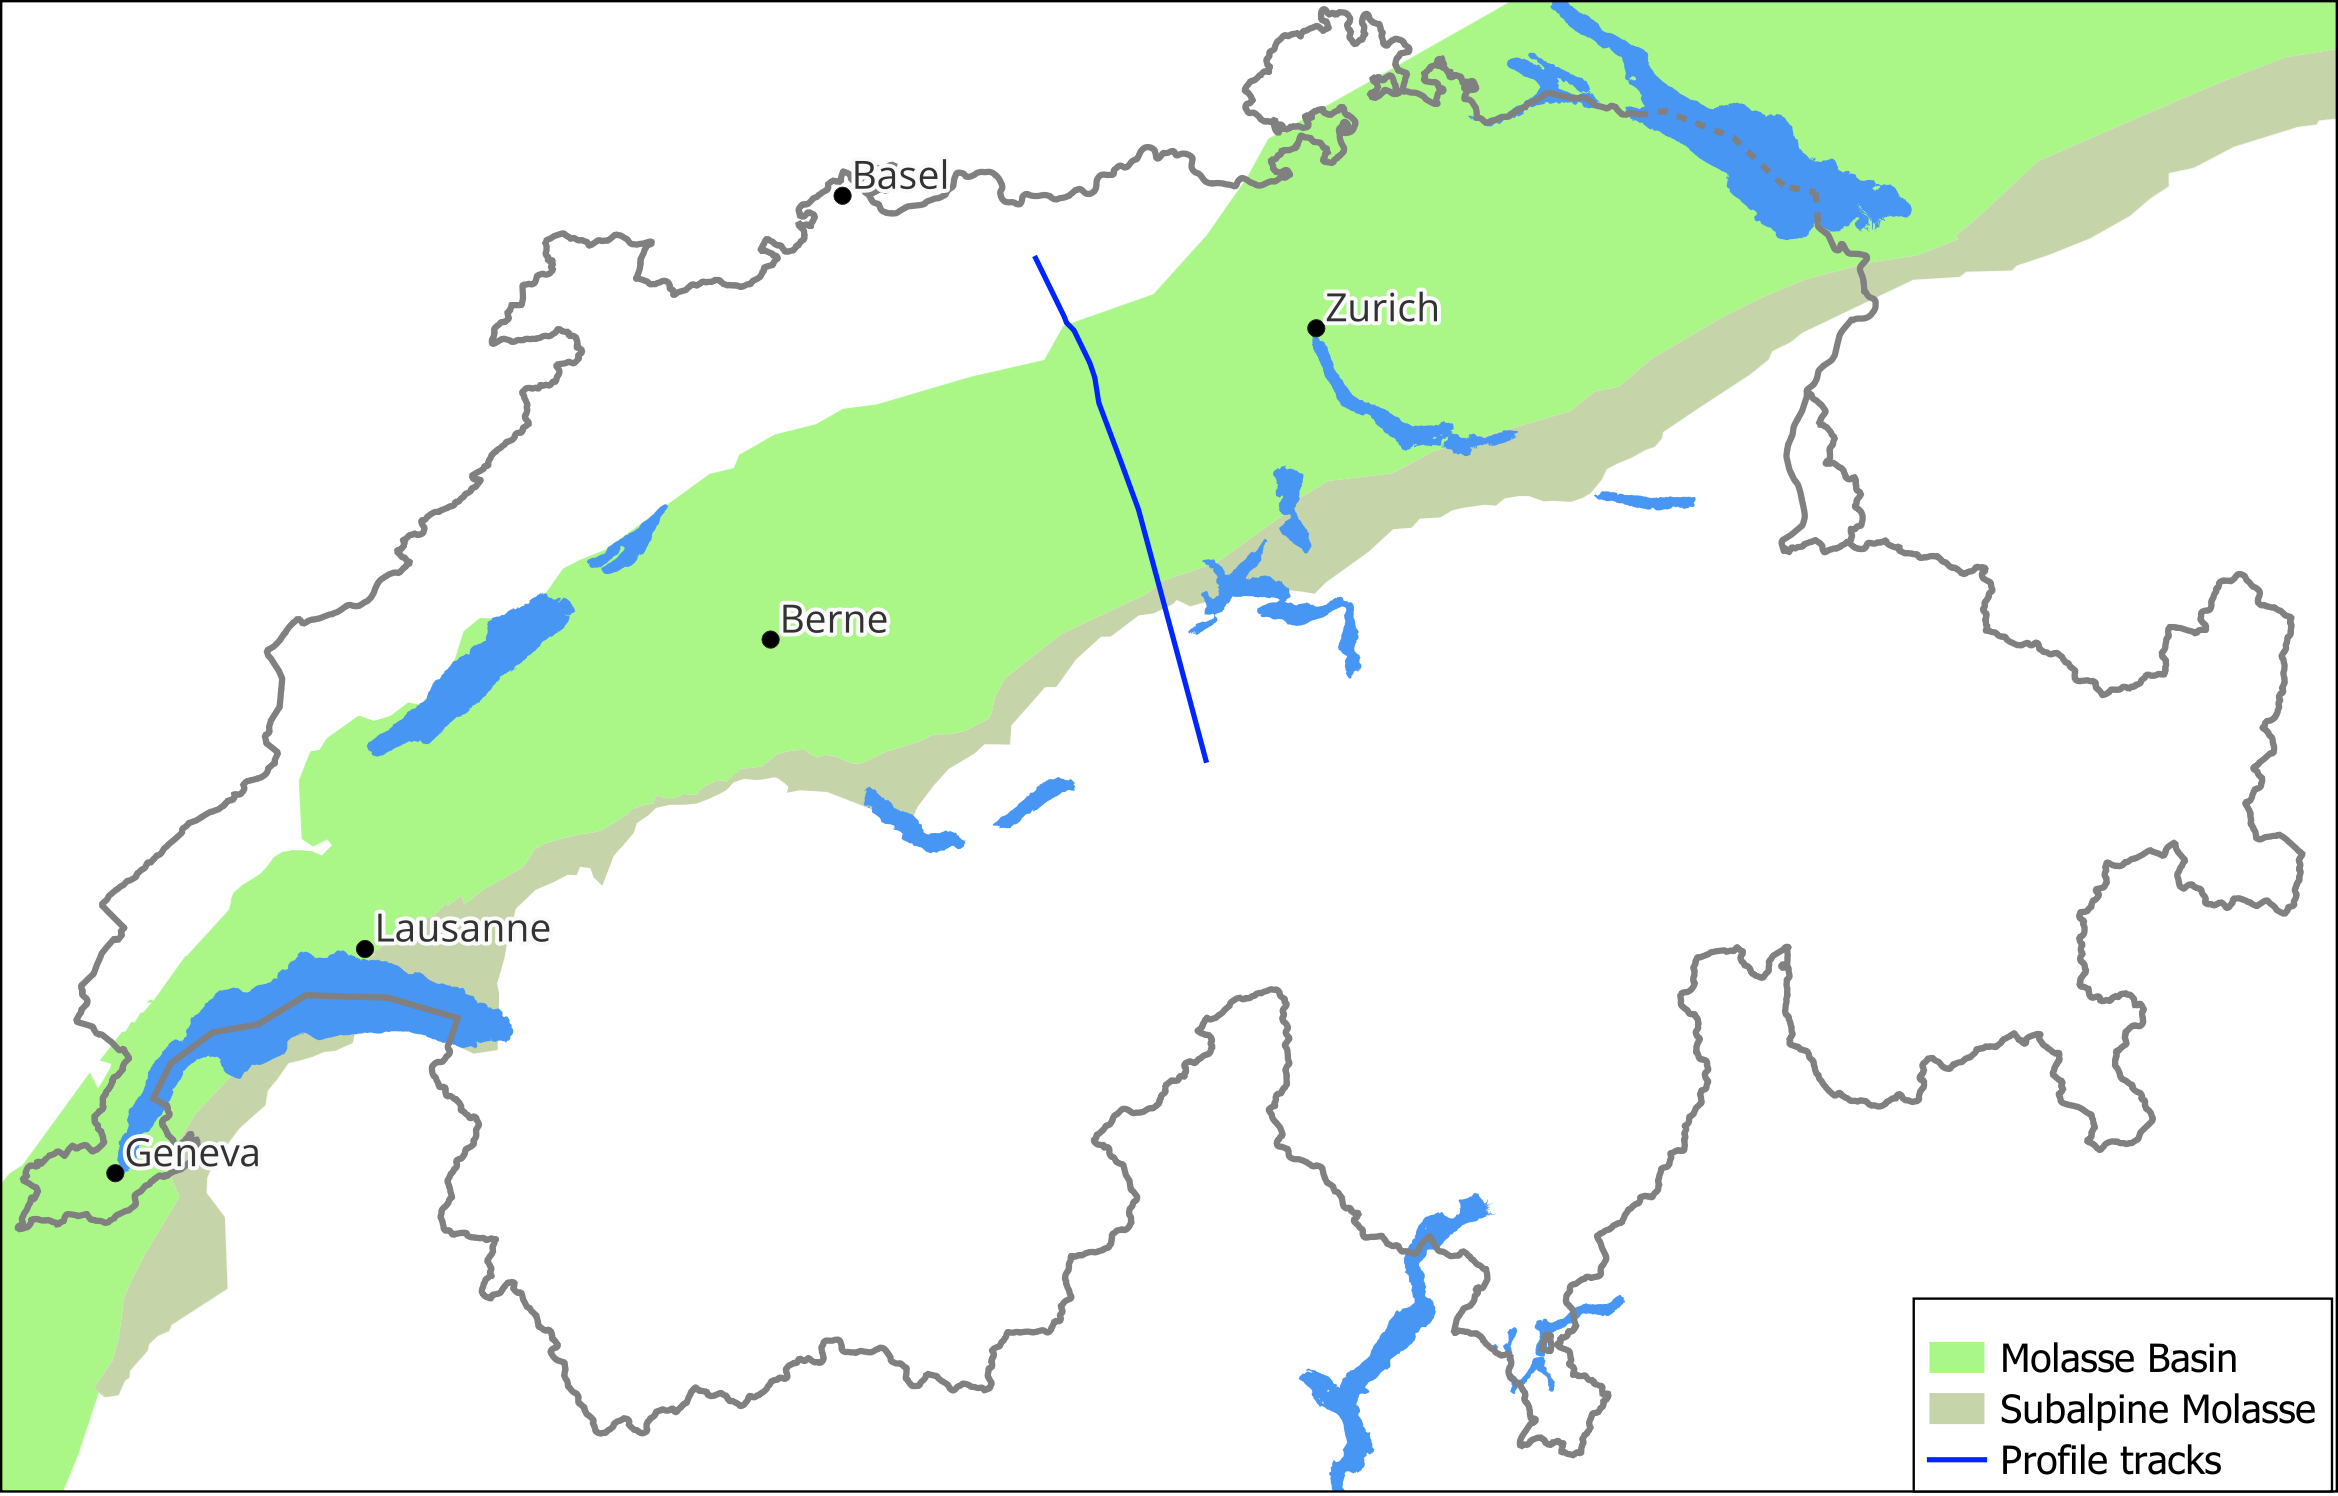
\includegraphics[width=0.8\textwidth]{img/molasse_basin.png}
    \caption{The extent of the molasse basin in Switzerland. The Subalpine Molasse is part of
    the molasse basin and forms its southern edge.}\label{fig:molasse_basin}
\end{figure}

\subsection{Geology}

The sediments filling the \SMB are the erosional debris
derived from the nearby Alps, with a thin cover of quaternary deposits. 
Grain size coarsens southward from mud/silt to gravel~\parencite{heim-geologie-bd1}. 
Because the sediments originate from individual catchments, they exhibit significant lateral variation
in clast composition and lithology,
which is particularly noticeable in the conglomerates and sandstones~\parencite{heim-geologie-bd1,Nesslau_Text,schlunegger-USM-facies-1997}.
This lateral variation complicates the interpretation and correlation of stratigraphic layers without the
broader context.

The molasse sediments are 
subdivided into units based on their prevalent depositional environment (marine vs. freshwater) and age.
This subdivision into \UMM and \USM
of Oligocene age, Upper Marine Molasse (\acro{OMM}) and \OSM
of Miocene age dates back to at least \textcite{heer-flora-1855} (\cref{fig:strati}).
The \UMM contains only mud-, silt- and sandstones, the \USM also contains pebbly conglomerates
and some freshwater carbonates~\parencite{heim-geologie-bd1}.
The subalpine molasse consists only of \UMM and \USM.
Throughout most of the basin, the molasse sediments unconformably lie on of the Mesozoic marine sediments of the 
northern Tethys \parencite{weissert-stoessl-2010}.
Along the Alpine front, the molasse stratigraphically overlays the 
flysch of the Helvetic nappe, but may also be overthrust by it. 
The reconstruction in \cref{fig:molasse_profile}
indicates that much of the subsurface structure is yet unknown.

\begin{figure}
    \centering
    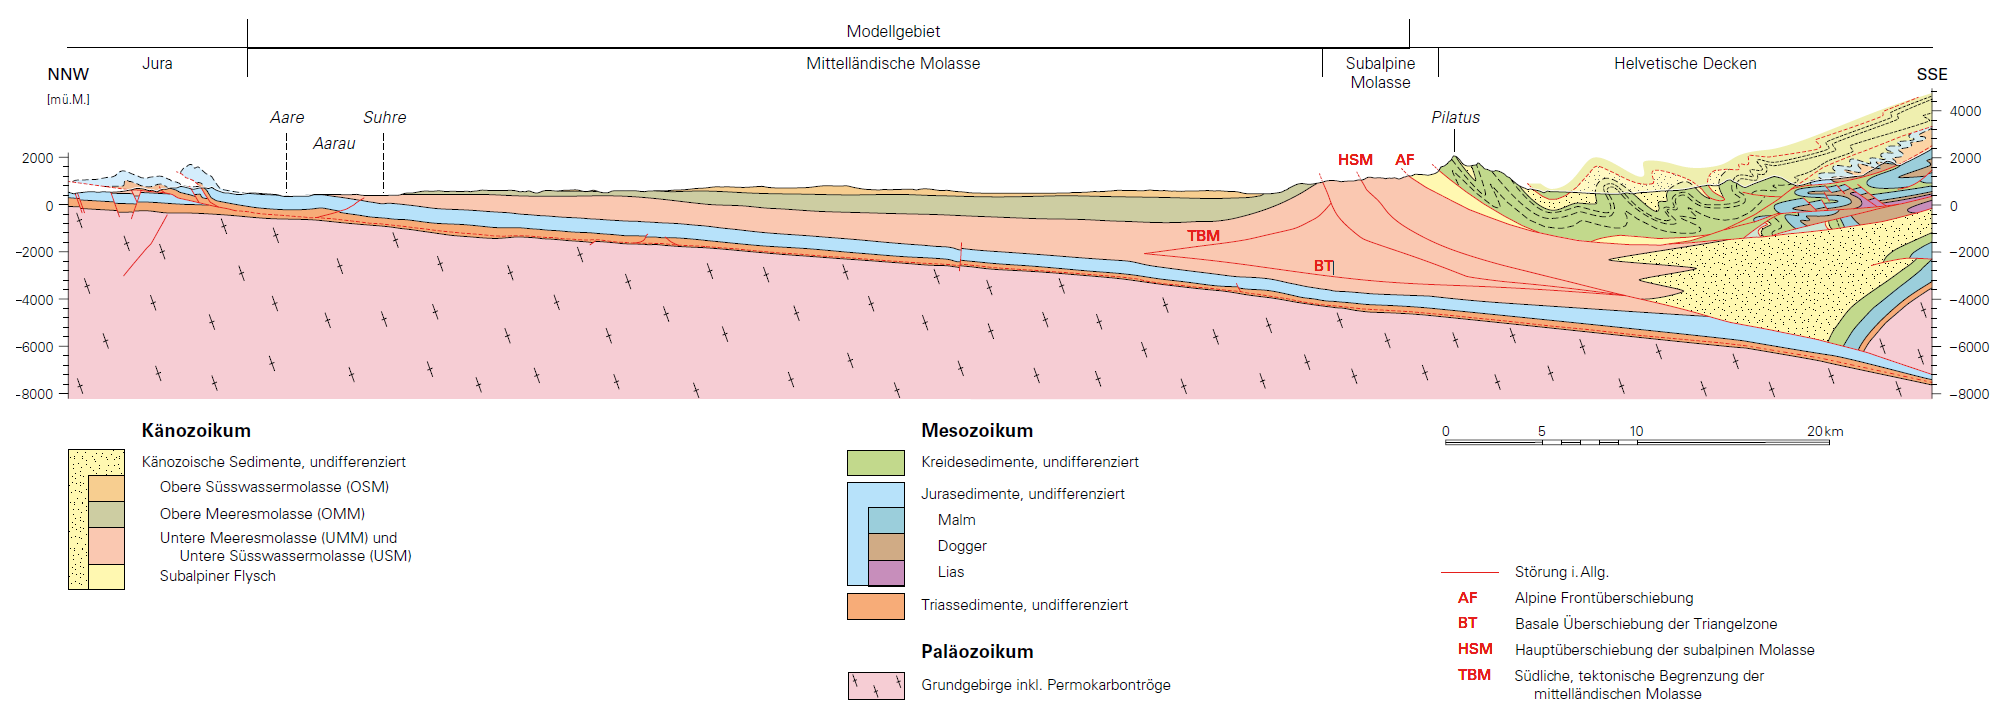
\includegraphics[width=\textwidth]{img/molasse_profile.png}
    \caption{Profile through the central SMB and bordering mountain 
    ranges~\parencite{geomol-2017}. Profile track shown in \protect\cref{fig:molasse_basin}.}\label{fig:molasse_profile}
\end{figure}

The division of \SMB units by facies is based
on macro fossils in some layers, assuming the fossil-poor surrounding
layers stem from the same depositional environment. \textcite{heim-geologie-bd1} introduced the important
qualification that the units are \emph{predominantly} (vorherrschend) of marine or freshwater
origin, rather than exclusively so. Various authors have reported such inconsistencies
between overarching unit classification and the actual depositional environment of the
sediments~\parencite{Linth_Text, Nesslau_Text}.

Determination of facies in these units is difficult, because fossils are sparse
and often not facies characteristic~\parencite{Nesslau_Text}. Additionally, many
units in the \SMB consist of mud- and siltstones, whose depositional environment
is difficult to determine using field methods alone~\parencite{Einsiedeln_Text}.
Recent works have used nanofossils to determine facies and age~\parencite{kempf_lower_2005}.

\begin{figure}
    \centering
    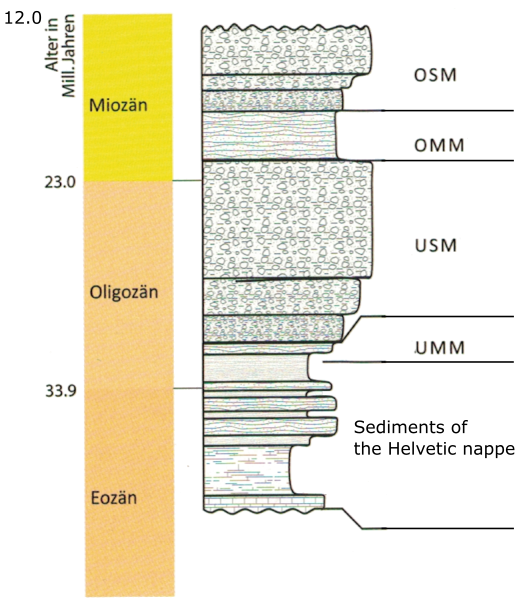
\includegraphics[width=0.3\textwidth]{img/molasse_simple_strati_mod.png}
    \caption{Stratigraphy and ages of the molasse sediments.
     Modified after \protect\textcite{weissert-stoessl-2010}.}\label{fig:strati}
\end{figure}

\section{Goals}

Advances in instrumental analyses for trace elements in rock samples,
e.g. \XRF or mass spectrometry, 
promise faster and easier access to geochemical analyses \parencite{ichikawa-xrf-2016,he_rapid_2018, he_determination_2019}.
This work investigates the utility of \XRF and \ICPMS for
measuring (trace) elements in mud- and siltstones, and the
use of previously published ratios of \acro{Sr}/\acro{Ba}, 
\acro{Cl}/\acro{Br} and \acro{S}/\acro{TOC} to characterize the
depositional environment of clay-rich sediments.
As a case study, samples from the Subalpine Molasse around Vorderthal, Switzerland are used~(\cref{fig:study_area}).

The experiments will:
\begin{itemize}
    \item Test whether \citeauthor{Worden_1996}'s \citeyear{Worden_1996} method 
    using the \acro{Cl}/\acro{Br} ratio is sufficient for a full classification.
    \item Test if the linear relationships for the \acro{Sr}/\acro{Ba}, 
    \acro{Cl}/\acro{Br} and \acro{S}/\acro{TOC} ratios determining the 
    fresh, brackish and marine
    water distinction established by \textcite{wei-2020} holds for our samples.
    \item Validate and if necessary update the geological map of the study 
    area~(\cref{fig:study_area}).
\end{itemize}

\begin{figure}[h]
\centering
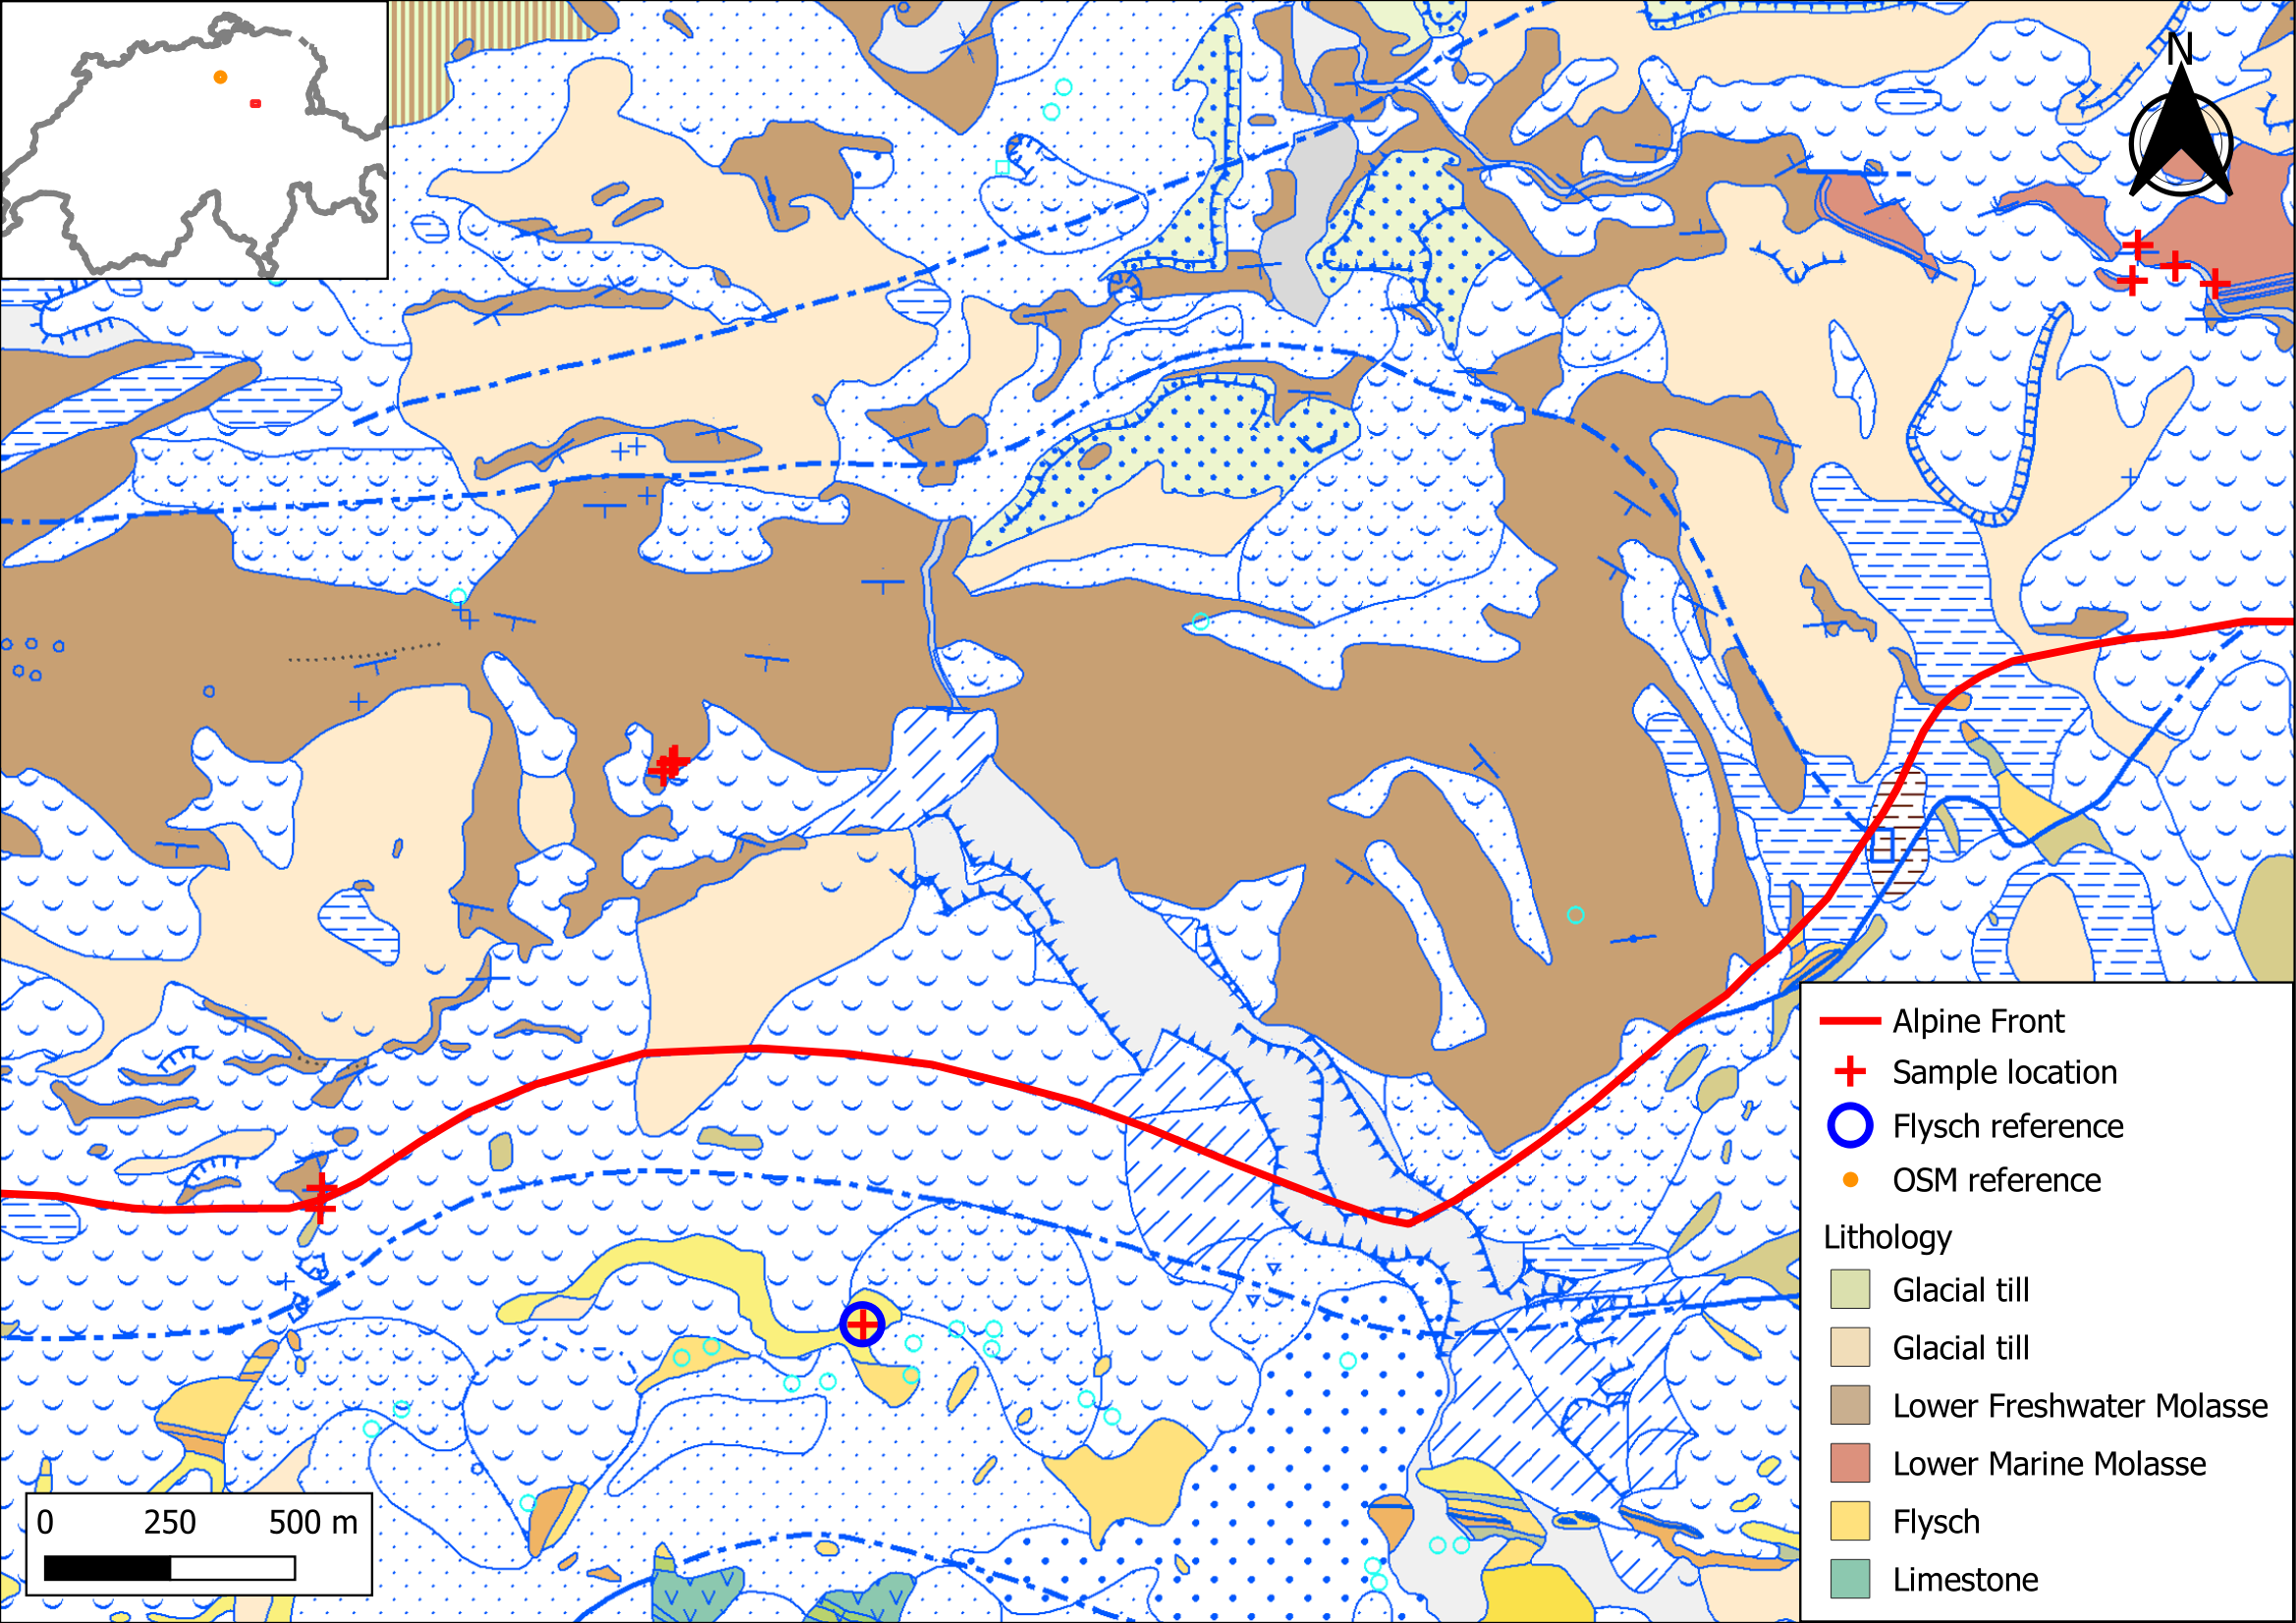
\includegraphics[width=.9\textwidth]{img/study_area.png}
\caption{The study area with sample locations. The \OSM reference location is at the orange
dot in the overview insert. Approx. GPS coordinates: 47.121420, 8.882903.
Modified from \citeauthor{swisstopo}.}\label{fig:study_area}
\end{figure}
\chapter{Methods}

Nine samples of mud- and siltstones were collected near the village
of Vorderthal along the tectonic contact between the SMB and the Helvetic 
nappe~(\cref{fig:study_area}). 
These were the primary samples for this study. In addition, one flysch sample from the Helvetic nappe
(marked in blue on the map in \cref{fig:study_area}), and one \OSM sample
from near Leimbach outside the main study area (orange dot in the
overview inset in \cref{fig:study_area}) were collected
as reference samples representing a marine and terrestrial
facies, respectively. The sample locations and corresponding samples
were designated ``JWL $x$'', where $x$ is an increasing number.

Concentrations of the elements \acro{Sr}, \acro{Ba}, \acro{Cl}, 
\acro{Br}, and \acro{S} as well as \TOC were determined using \XRF, \ICPMS
and the TOC-only mode of isotope-ratio mass spectrometry (\acro{IRMS}).
\XRF should be able to determine all target elements except carbon~\parencite{ichikawa_solid_2023}, \ICPMS
can measure trace metals and, with appropriate digestion methods, halogens~\parencite{he_rapid_2018}. 
IRMS combustion analysis is specific to \TOC~\parencite{irms}.
Using several methods for each element enables cross-validation 
of the results, and helps identify the most suitable method for individual elements.

The computed concentration ratios for Sr/Ba and S/TOC were compared against published classification thresholds
by \textcite{berner-raiswell-1983,wei-2020}. An approximate best fit threshold was computed
using the Receiver Operating Characteristic (ROC) curve approach \parencite{fawcett-roc-2006}.
In all cases, samples are classified as marine when their trace-element ratio exceeds a specified threshold.
The ROC algorithm tests which of the computed ratios in our dataset best reproduces the classification 
from the geological map.
Because of the mathematical properties of ROC curves, selecting the best fit threshold
using Youden's J statistic yields an approximation that minimizes classification errors \parencite{youden-index-2019}.

\section{Rock powder preparation}

All measurement methods use fine rock powder as the starting material. 
The samples were therefore processed following a protocol adapted from \textcite{ichikawa_solid_2023}:
\begin{enumerate}
    \item Samples were first dried at 40\degree C for at least one week.
    
    \item Approximately 60\,g of the samples were crushed and then milled for 4 minutes in a
    tungsten carbide vessel on a vibrating mill. 
    Milling was extended to 8 minutes when necessary to achieve sufficiently fine powder.
    
    \item The powders were dried at $100 \pm 5$\degree C for at least 24\,h and
    cooled in a desiccator, and then stored in closed but not sealed containers.
\end{enumerate}


\section{X-Ray Fluorescence (\XRF)}

\XRF measures the characteristic fluorescence of atoms caused by irradiation with X-rays.
Reliable measurements require the irradiated sample to be homogenous across
the entire analysed volume. Homogeneity is achieved by using
fine rock powder as the sample. This powder can either be pressed into a pellet
together with a binding agent, or it can be fused with a borate-based flux to
produce glass beads~\parencite{ichikawa_solid_2023}.
The high temperatures required to melt the borate flux cause volatiles like
halogens and sulphur to evaporate.
To preserve all volatiles, for this study we used powder pellets. 

To obtain consistent, reproducible results, the grain sizes in samples should be smaller than the analytical 
depth and the thickness of the pellet should exceed the escape depth~\parencite{ichikawa_solid_2023}.
The escape depth is always smaller than the analytical depth, which can be obtained from
standard tables~(cf.~\cref{tab:xrf-analytical-depth}).
A powder pellet suitable for the XRF unit at \ETH is a disc
approximately 4\,cm in diameter and 3-4\,mm thick (\cref{fig:xrf-pellets}). The 4\,mm thickness of the pellets
is sufficient for our target elements.

% For accurate and repeatable measurements \textcite{ichikawa_solid_2023} suggested
% adjusting the powder grain size and the pellet's surface smoothness to the elements of
% interest.
% The \emph{escape depth} or \emph{analytical depth} of fluorescent X-rays depends on their wavelength and the 
% average density of the material of the pellet. 
% \emph{Escape depth} refers to the maximum depth from within the pellet that fluorescent radiation of
% a specific wavelength can still escape instead of being absorbed by heavy atoms in the sample.
% \emph{Analytical depth} refers to how deeply the irradiating X-rays can penetrate the sample.
% Both of these are governed by the properties of the sample material and the elements we want to measure.

% How far X-rays can penetrate a material
% is governed by the Lambert-Beer law

% \begin{equation}\label{eq:lambert}
%     I = I_0 \exp(-\mu_\lambda \cdot \rho \cdot d)
% \end{equation}

% where $I$ is the intensity of the X-rays of initial intensity $I_0$ after penetrating a material
% to depth $d$ in a sample of average density $\rho$ 
% with a mass absorption coefficient of $\mu_\lambda$. Rearranging \cref{eq:lambert} and setting
% $I=I_0/2$ yields a formula for the \emph{half-thickness}, the depth at which the initial intensity 
% has halved:

% \begin{equation}
%     \frac{I_0}{2} = I_0 \exp(-\mu_\lambda \cdot \rho \cdot d) \Leftrightarrow d_{0.5} = \frac{\ln 2}{\mu_\lambda\cdot\rho}
% \end{equation}

% \textcite{ichikawa_solid_2023} estimated the escape depth to be four times the half-thickness.
% For most analyses it is sufficient to estimate the analytical depth. Therefore, using tabled values for
% the mass absorption coefficient and average densities for common rock types is acceptable (cf.~\cref{tab:xrf-analytical-depth}).


\begin{figure}[b]
  \nopagebreak
  % Left side: The Figure
  \begin{minipage}[b]{0.45\textwidth}
    \vfill
    \centering
    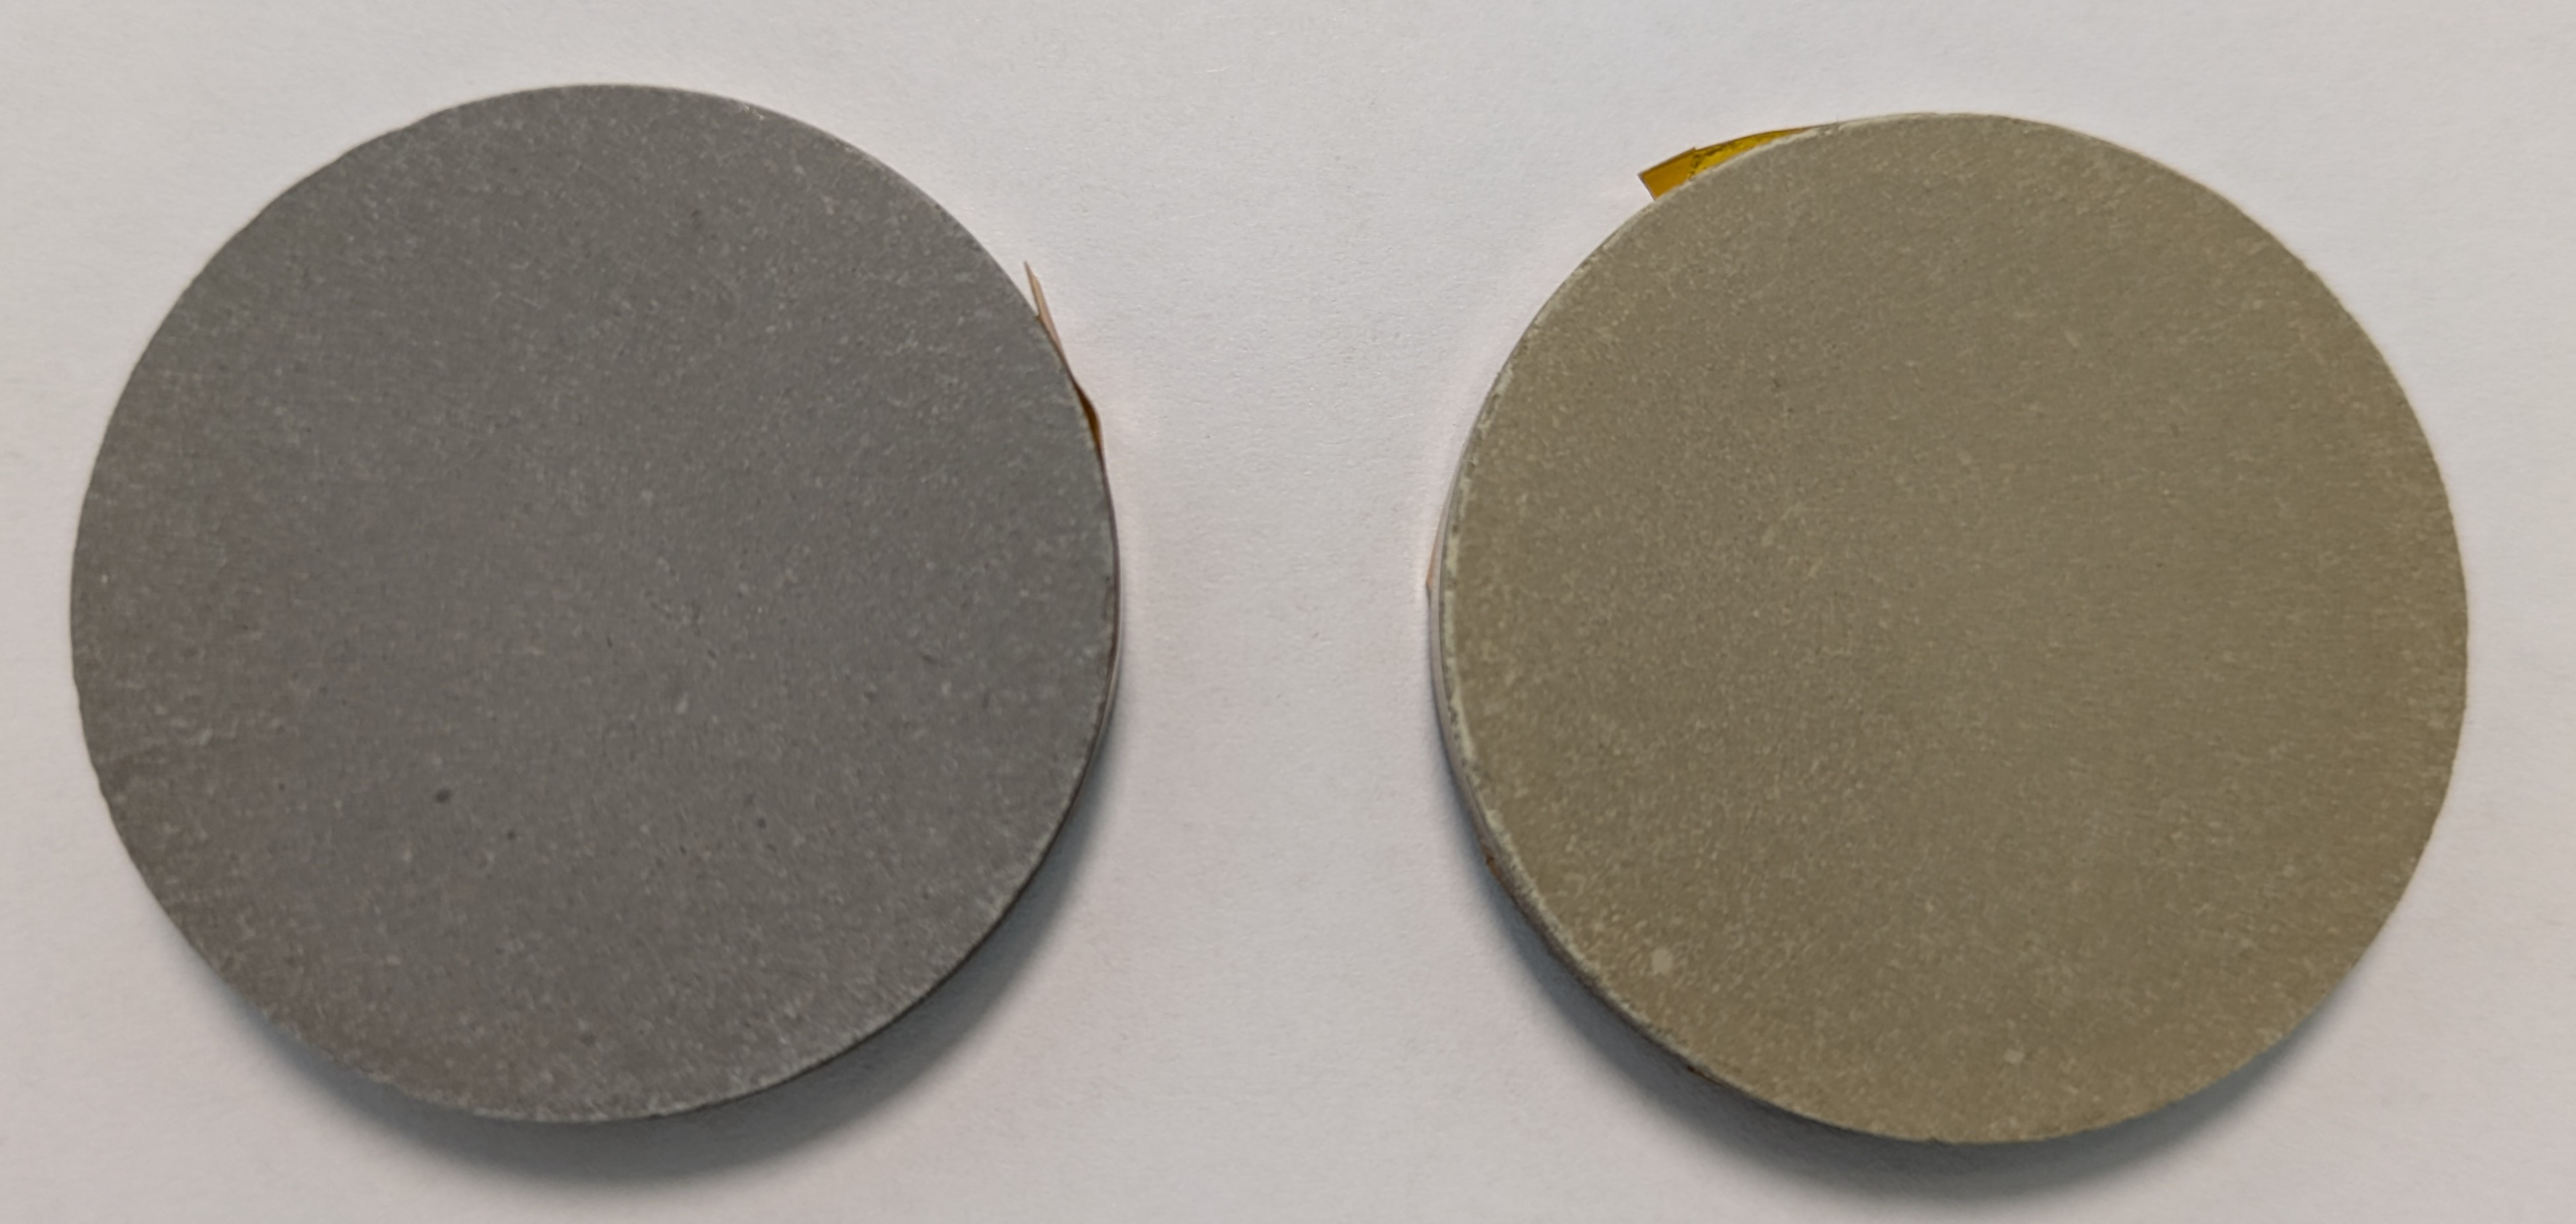
\includegraphics[width=0.95\textwidth]{img/xrf_pellets.jpg}
    \captionsetup{width=0.95\linewidth}
    \caption{Pellets for rock samples JWL 1 and JWL 2.}
    \label{fig:xrf-pellets}
  \end{minipage}
  \hfill % Adds horizontal space between the minipages
  % Right side: The Table
  \begin{minipage}[b]{0.48\textwidth}
    \centering
    \captionsetup{width=0.95\linewidth}
    \captionof{table}{Analytical depths for elements of interest, estimated with Bruker's online
    ``XRF Check'' calculator \parencite{bruker-xrf-check}.}
    \label{tab:xrf-analytical-depth}
    \begin{tabular}[b]{ll}
        \toprule
        \textbf{Element} & \textbf{Analytical depth [$\mu$m]} \\\midrule
        Ba &  4500 \\
        Br & 427\\
        Cl & 5.34 \\
        S & 3.77 \\
        Sr & 660 \\        
        \bottomrule
    \end{tabular}
  \end{minipage}
\end{figure}

\subsection{Sample preparation}
 
Because we did not have access to a means to control the grain size of the powders we produced, 
we used a standard protocol used for the preparation of powder \XRF pellets at \ETH:

\begin{enumerate}
    \item Sample powder and binding agent were mixed at a mass ratio of 8:2 for
    a total of 10\,g. 
    \item The mixture was homogenized in 
    a shaker for 4 minutes; in few cases 8 minutes were required.
    \item The mixture was pressed into pellets of 40\,mm diameter with a stepwise pressure increase  
    of 100, 200, 300, 400, 450\,bar, holding each pressure for 20 seconds without releasing pressure
    between steps.
\end{enumerate}

Some samples did not form stable pellets at the 8:2 ratio. In those cases powder:binder
ratios of 7:3 and 6:4 were tried and yielded stable pellets.
Two pellets were produced and analysed for each rock sample, 

\subsection{Measurements}

All samples were analysed using a Bruker Tiger S8 WDXRF unit\footnote{\url{https://www.bruker.com/en/products-and-solutions/elemental-analyzers/xrf-spectrometers/s8-tiger.html}}
(20kV-60kV) with a Rhodium anode to determine
concentrations of \acro{Cl}, \acro{Br}, \acro{Sr}, \acro{Ba} and \acro{S}.
Because the instrument was not yet calibrated with certified reference materials
and certified rock standards for the rocks we analysed were not available, we used the
fundamental parameter method~\parencite{ichikawa_solid_2023}.
Therefore, the accuracy of the results is likely less than it could be. 

For each measurement, the analytical software reports all elements above their respective detection limits.
It also provides the \emph{Compton ratio} as an indication
of how reproducible, and thus how representative of the sample, that measurement is estimated to be.

\section{ICP mass spectrometry}

\ICPMS requires samples to be in liquid form so they can be aerosolized 
and injected into the plasma chamber where they are vaporized and ionized 
before entering the mass spectrometer.
For rock samples, digestion with \acronym{HF}{hydrofluoric acid} is commonly used 
to produce the required solution for trace metal analysis~\parencite{hu-digestion-2014}. 
\textcite{he_rapid_2018} also applied this
method to extract halogens. In addition, they proposed \acronym{\ambif}{ammonium bifluoride}
as a solid flux that improves halogen retention and reduces the impact of 
aggressive acids on the instrument~\parencite{he_determination_2019}.

We used \acro{HF} digestion to obtain concentrations of all elements
that remain stable during the digestion process. Because halogens \emph{are} volatile and
leave the resulting slurry, 
we also used \ambif\ digestion to accurately measure \acro{Cl} and \acro{Br}, following the
procedure described by \textcite{he_determination_2019} as closely as possible.

For both digestion methods, we measured the two common 
rock standards BCR-2 and BHVO-2 for quality control~\parencite{bcr2, bhvo2}.
Additionally, for the digestion with \acro{\ambif} we prepared several
reagent blanks containing only \acro{\ambif} to quantify and correct for 
impurities in the reagent.

\subsection{Sample preparation}

\subsubsection{\ambif\ digestion}
\begin{enumerate}
\item 100\,mg of sample were weighed into a Teflon vial.
\item 400\,mg of \ambif\ were added into the vial.
\item The mixture was heated to 200-220\degree C for 2\,h in closed, but not sealed vials.
After cooling, this should result in a solid digestion cake.
\item This residue was washed and partially dissolved with 5\,ml 5\% NH$_3$ solution.
\item The resulting mix of slurry and solution was centrifuged for 10 minutes.
\item The supernatant was taken as the solution for \ICPMS.
\end{enumerate}

\textcite{he_determination_2019} did not provide enough detail how to move from step 3 to step 6. 
They only state ``The digestion cake was diluted by 5\% v/v NH$_4$OH
solution to 25 g after cooling.''~\parencite[p. 8110]{he_determination_2019}.
This presumes that the halogens remain in the digestion cake, and not in the atmosphere of the vial.
The vial volume (7\,ml) makes dilution to 25\,g total mass impossible. 
Consequently, the cake would have to be transferred to a 
larger vessel. This can lead to loss of material, and thus measurement uncertainty.

Because \ambif\ digestion is an untested technique at \ETH, we prepared three vials each for the \OSM and flysch
samples to quantify the measurement variability for identical rock samples.

% \begin{figure}
%     \centering
%     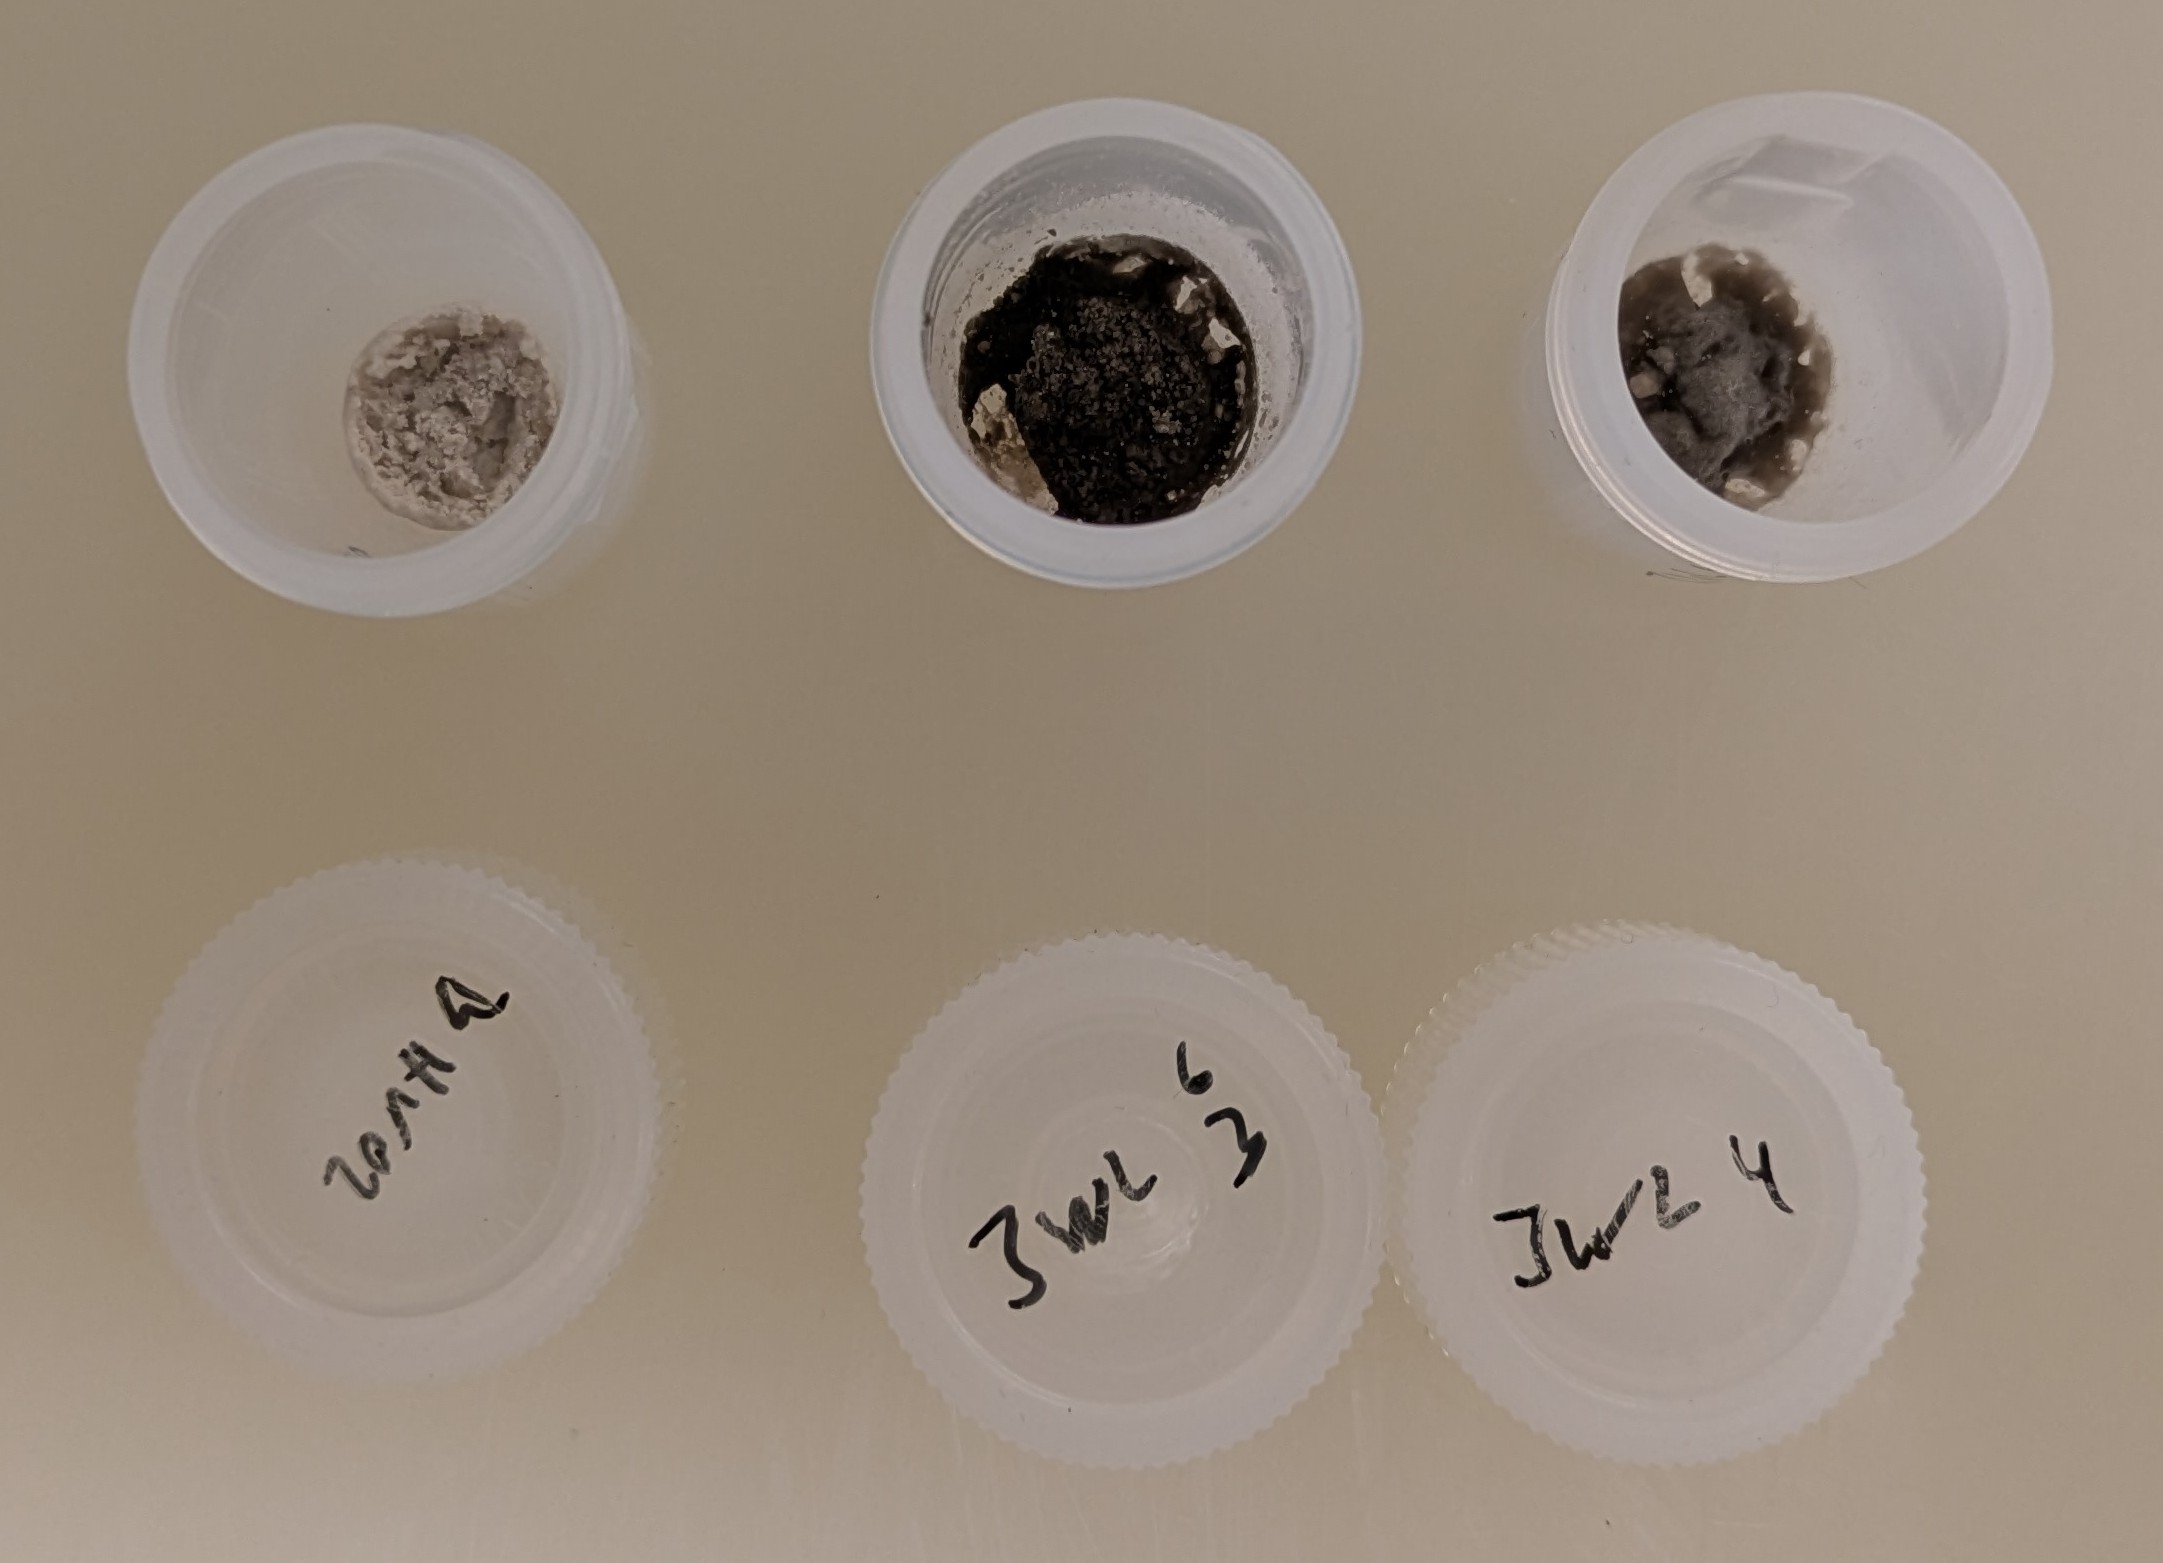
\includegraphics[width=0.45\textwidth]{img/NH4_samples.jpg}
%     \caption{Photograph of some sample vials with the digestion cake after step 3. }
%     \label{fig:NH4-samples}
% \end{figure}

\subsubsection{HF digestion}

The protocol for \acro{HF} digestion is similar to the one for \ambif:

\begin{enumerate}
\item 5\,mg of sample were weighed into a Teflon vial.
\item A mixture of concentrated \acro{HF} and concentrated nitric acid (\acro{HNO$_3$}) 
    was added to the sample vial.
\item The mixture was heated on a hotplate to 200-220\degree C for two days.
\item The resulting solution was diluted with 2\% nitric acid and directly used for \ICPMS.
\end{enumerate}

\subsection{Measurements}

Both sets of samples were measured following the standard procedure at \ETH.
Blank solutions were measured first to define the instrumental background.
Then internal reference standards were measured to allow drift correction of later measurements.
The rock samples were measured in batches of five, and after each batch
the reference standards were measured again to detect instrument drift. 


\section{Total organic carbon (\acro{TOC})}

To determine \TOC, inorganic carbon must first be removed from the samples. 
After carbonate removal, the samples are combusted in an oxygen atmosphere. 
The resulting CO$_2$ is measured and attributed entirely to \TOC~\parencite{irms}.

\subsection{Sample preparation}

For each rock sample, two pellets were prepared.
Sample preparation followed the protocol below:

\begin{enumerate}
    \item 100\,mg of sample were weighed into a tin boat.
    \item The samples were soaked with HCl for several days to remove all carbonates.
    \item The residue was dried and packed into fresh tin boats and pressed into small pellets.
\end{enumerate}


\subsection{Measurements}

The pellets were combusted at high temperature in an oxygen
atmosphere. Under these conditions, all organic carbon oxidizes to CO$_2$.
The amount of resulting CO$_2$ was measured with \acro{IRMS} and converted
back to carbon concentrations in the samples.

\chapter{Results}\label{sec:results}

The geological map of the study area \parencite{Linth_Map} provides a classification for 
all sample locations. Samples mapped as \USM are classified as freshwater,
\UMM as marine~(cf. fig.~\ref{fig:study_area}). The flysch and \OSM samples are marine and 
freshwater respectively \parencite{Linth_Text,gubler_2009e}. 

The XRF instrument reports the \emph{Compton ratio} as an indicator for the reproducibility,
and thus reliability, of the measurements. For most samples the instrument reports moderate to low 
Compton ratios (\cref{tab:sr-ba-table}), 
suggesting that the results should be interpreted only qualitatively.
Quantitative interpretation should be approached with caution.

\section{Cl/Br}

The \XRF measurements for \acro{Cl} were inconsistent. \acro{Cl} was detected in only six samples,
and only one sample yielded \acro{Cl} in both pellets. 
\acro{Br} was not detected in any sample. 

The \ICPMS measurements of halogens following the \ambif\ method of \textcite{he_determination_2019}
produced inconsistent results. Throughout the measurement cycle, instrument sensitivity
decreased by approximately two orders of magnitude (\cref{fig:halogen-sensitivity}).

When the raw \acro{Cl} counts of the standard solutions are plotted
against the respective concentrations of 10, 100 and 1000\,ppb Cl, the linear regression line does not
pass through (0,0), instead it shows a large positive intercept. Subtracting the regression intercept
from the measured counts, the \acro{Cl} counts are comparable to \acro{Br}~(\cref{fig:cl-br-counts-run1}).
The reagent blanks containing only \ambif\ also show high Cl counts~(\cref{fig:cl-br-blanks}).
This indicates a systematic background signal for Cl.

\acro{Cl} (after correction) and \acro{Br} showed different results across the three standard solutions
of 10, 100 and 1000\,ppb Cl and Br throughout the measurement run~(\cref{fig:cl-br-counts}).
At the beginning, the counts for \acro{Br} increased linearly with concentration as expected, 
while the trend for \acro{Cl} was not quite as clear~(\cref{fig:cl-br-counts-run1}).
At the end of the measurement run, after all samples had been measured, \acro{Br} still displayed a clear linear
increase, while \acro{Cl} appeared more scattered and showed no linear trend~\Cref{fig:cl-br-counts-run3}.

We observed significant instrument corrosion after the measurements and attribute the
decline in instrument sensitivity to this damage. 
Therefore, the results cannot be considered reliable, and will not be discussed further.

\begin{figure}[]
  \nopagebreak
  % Left side: The Figure
  \begin{minipage}[t]{0.48\textwidth}
    \vspace{0pt}
    \centering
    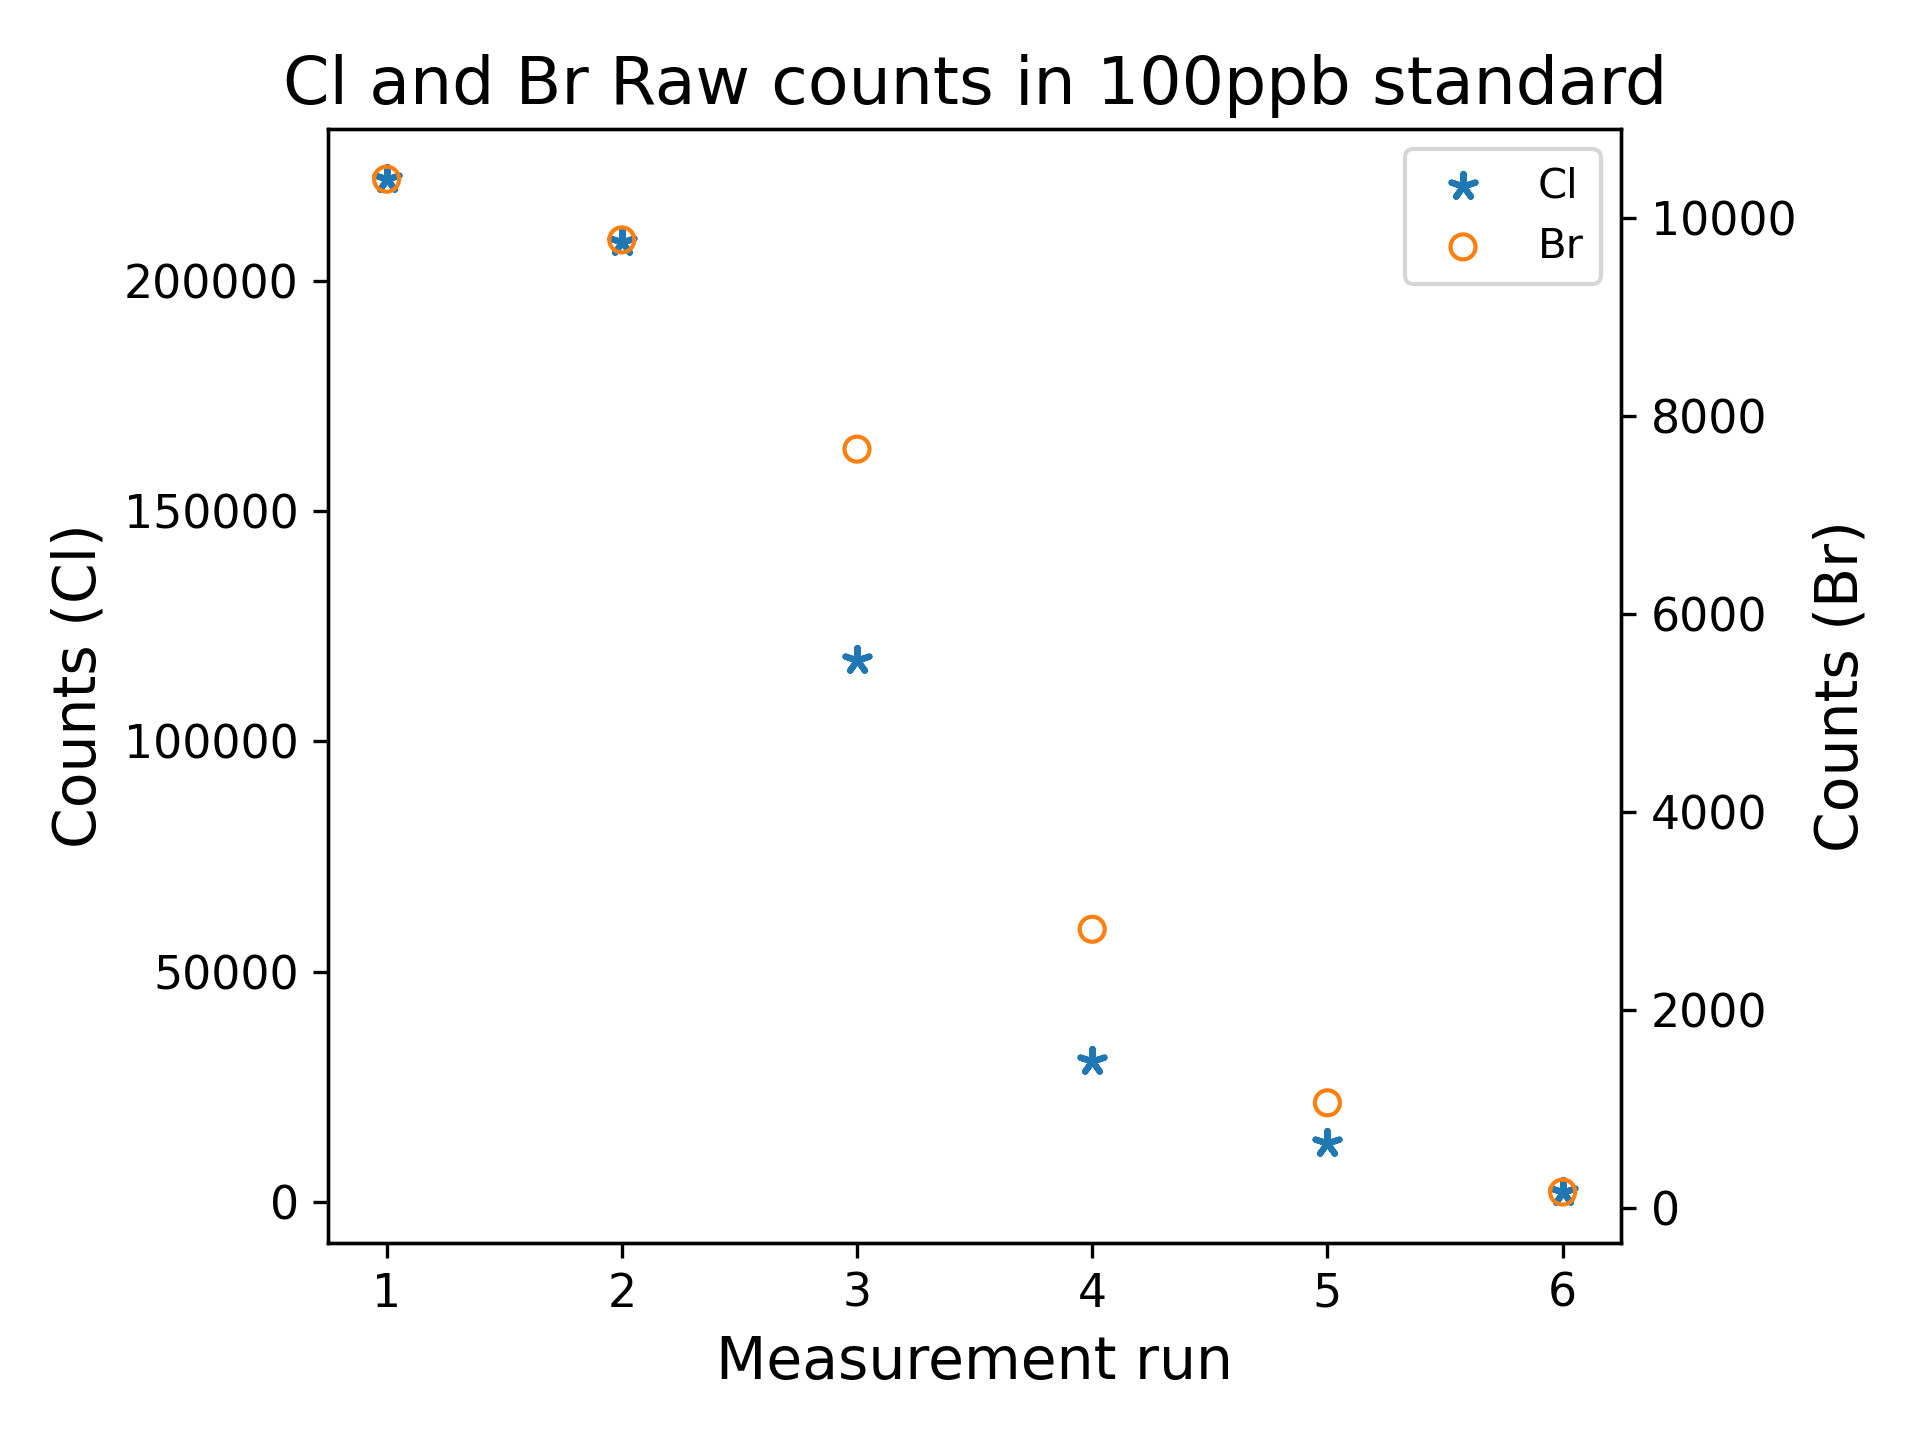
\includegraphics[scale=0.47]{img/icpms_halogen_sensitivity.png}
    \captionsetup{width=0.95\linewidth}
    \caption{Counts for Cl and Br throughout the measurement run. The measured solution
    is always with 100\,ppb Cl and Br.}
    \label{fig:halogen-sensitivity}
  \end{minipage}
  \hfill % Adds horizontal space between the minipages
  % Right side: The Table
  \begin{minipage}[t]{0.48\textwidth}
    \vspace{0pt}
    \centering
    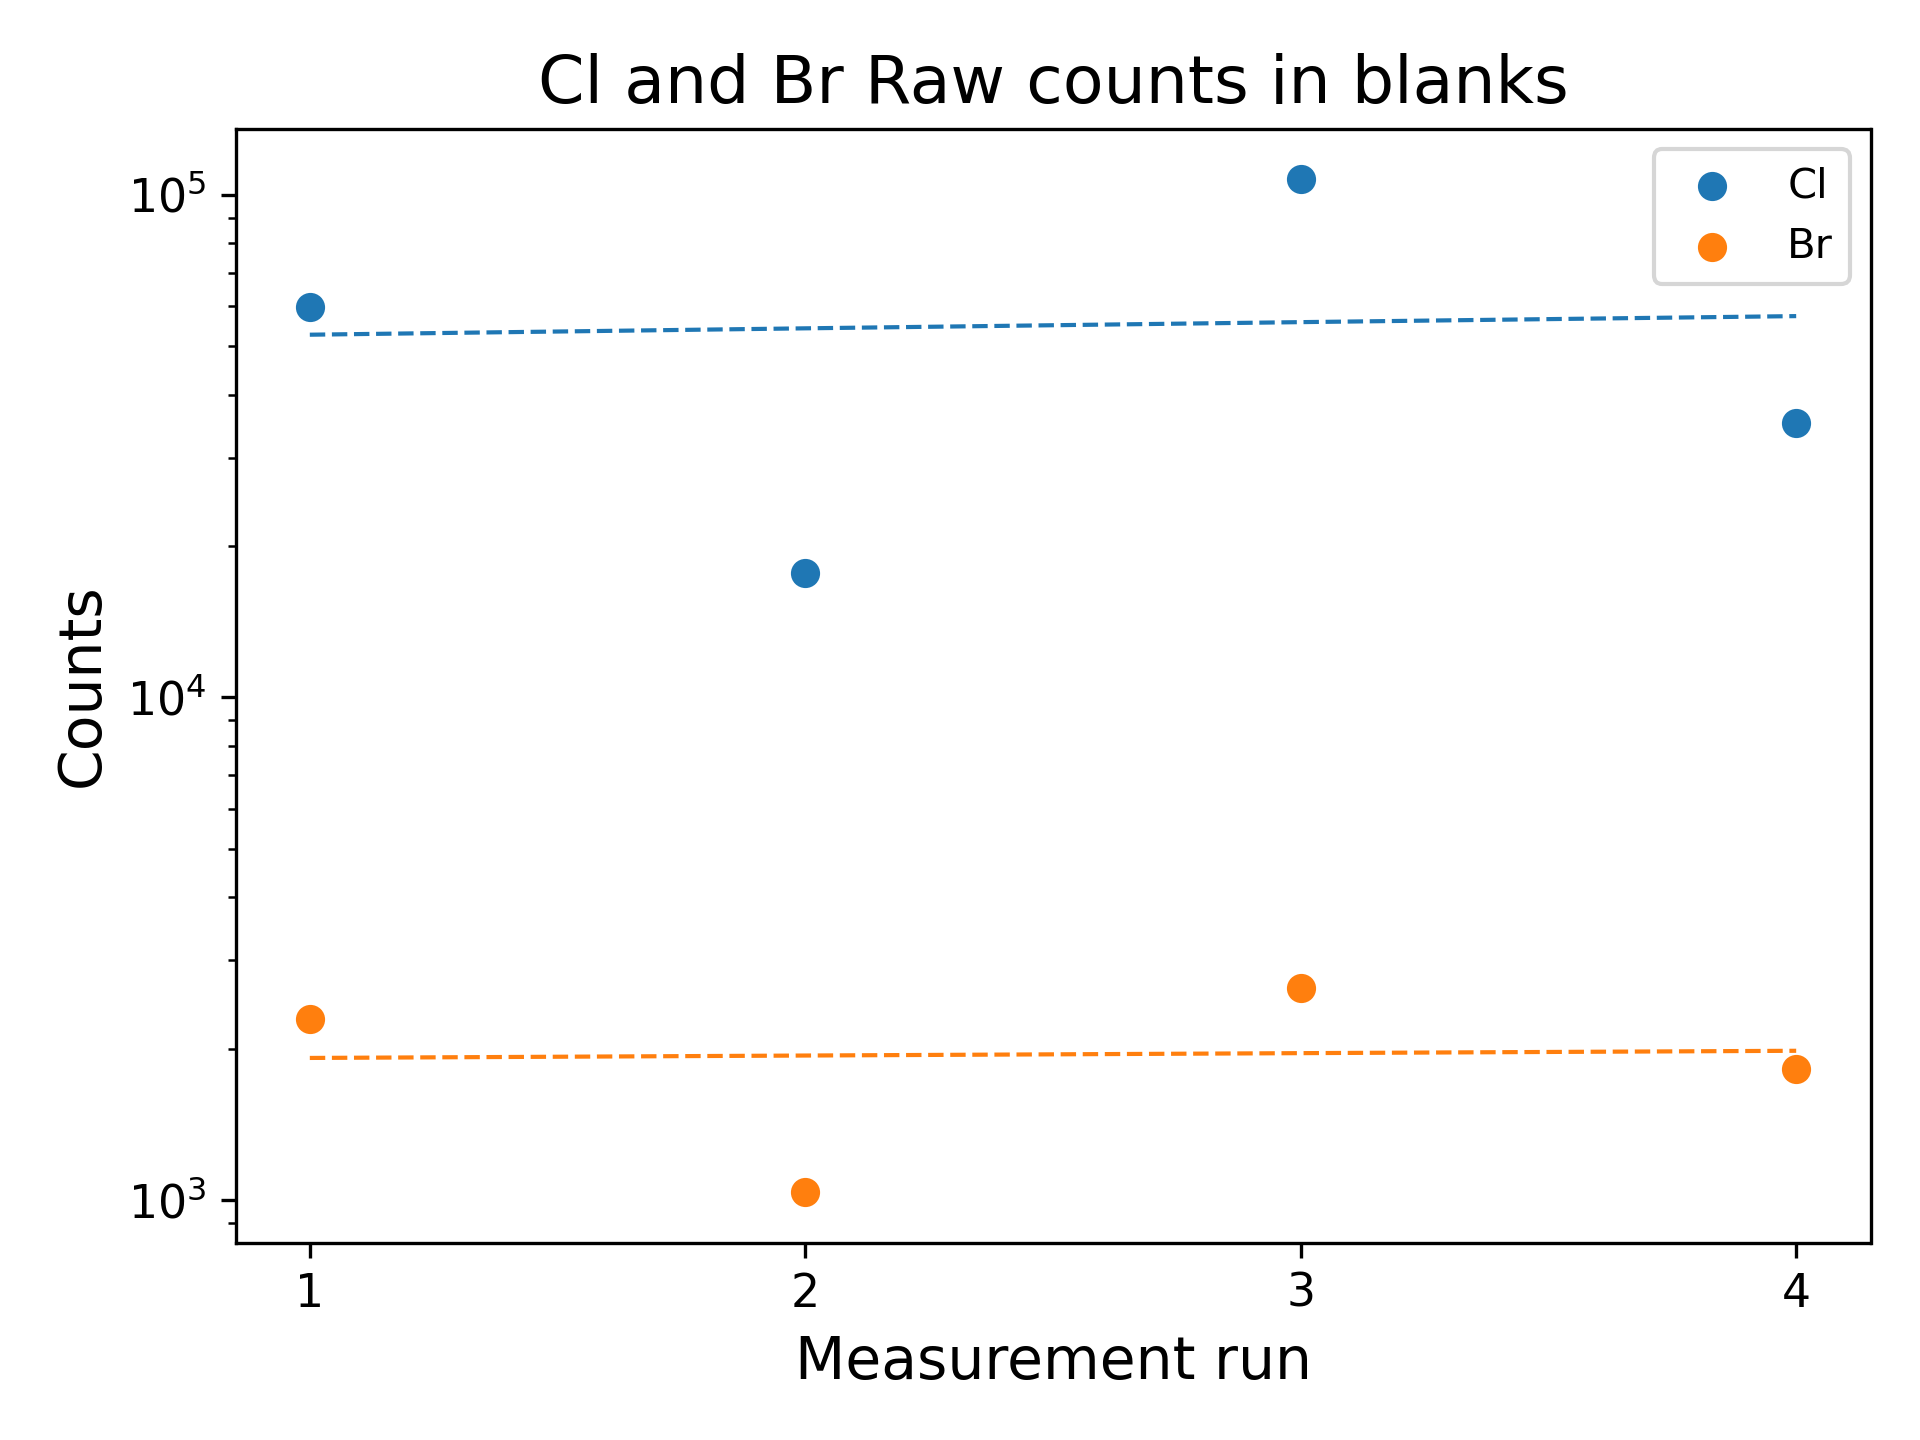
\includegraphics[scale=0.47]{img/cl_br_blanks.png}
    \captionsetup{width=0.95\linewidth}
    \caption{Measurement of \ambif\ reagent blanks show that Cl counts are systematically higher than Br.}
    \label{fig:cl-br-blanks}
  \end{minipage}
\end{figure}


\section{Sr/Ba}

\XRF yielded \acro{Sr} and \acro{Ba} concentrations for all samples except for the \OSM
reference sample, in which no \acro{Ba} was detected.
The \acro{Ba} measurements had uncertainties of approximately 10\%, while
the uncertainties for \acro{Sr} were approximately 0.5\% (\cref{tab:sr-ba-table}).
\ICPMS yielded \acro{Sr} and \acro{Ba} concentrations for all samples. 
Compared to \XRF, the \ICPMS concentrations for \acro{Ba} were approximately 50\% lower,
while \acro{Sr} was typically
50-100\,ppm higher. The uncertainties were 13.7\% for \acro{Ba} and 7\% for \acro{Sr}~(\cref{tab:sr-ba-icpms-table}).

\Cref{fig:sr_ba_crossplot} shows \acro{Sr} over \acro{Ba} for both methods.
The data points are colour-coded based on the classification in \parencite[\protect\cref{fig:study_area}]{Linth_Map}.
This classification
corresponds to \emph{marine} for \UMM and Flysch, and \emph{freshwater} for \USM and \OSM.
This classification highlights JWL 1 as an outlier compared to the other freshwater samples.

\begin{figure}
    \centering
    \subfigure[Standard Cl and Br counts \emph{before} measuring samples.\label{fig:cl-br-counts-run1}]{
        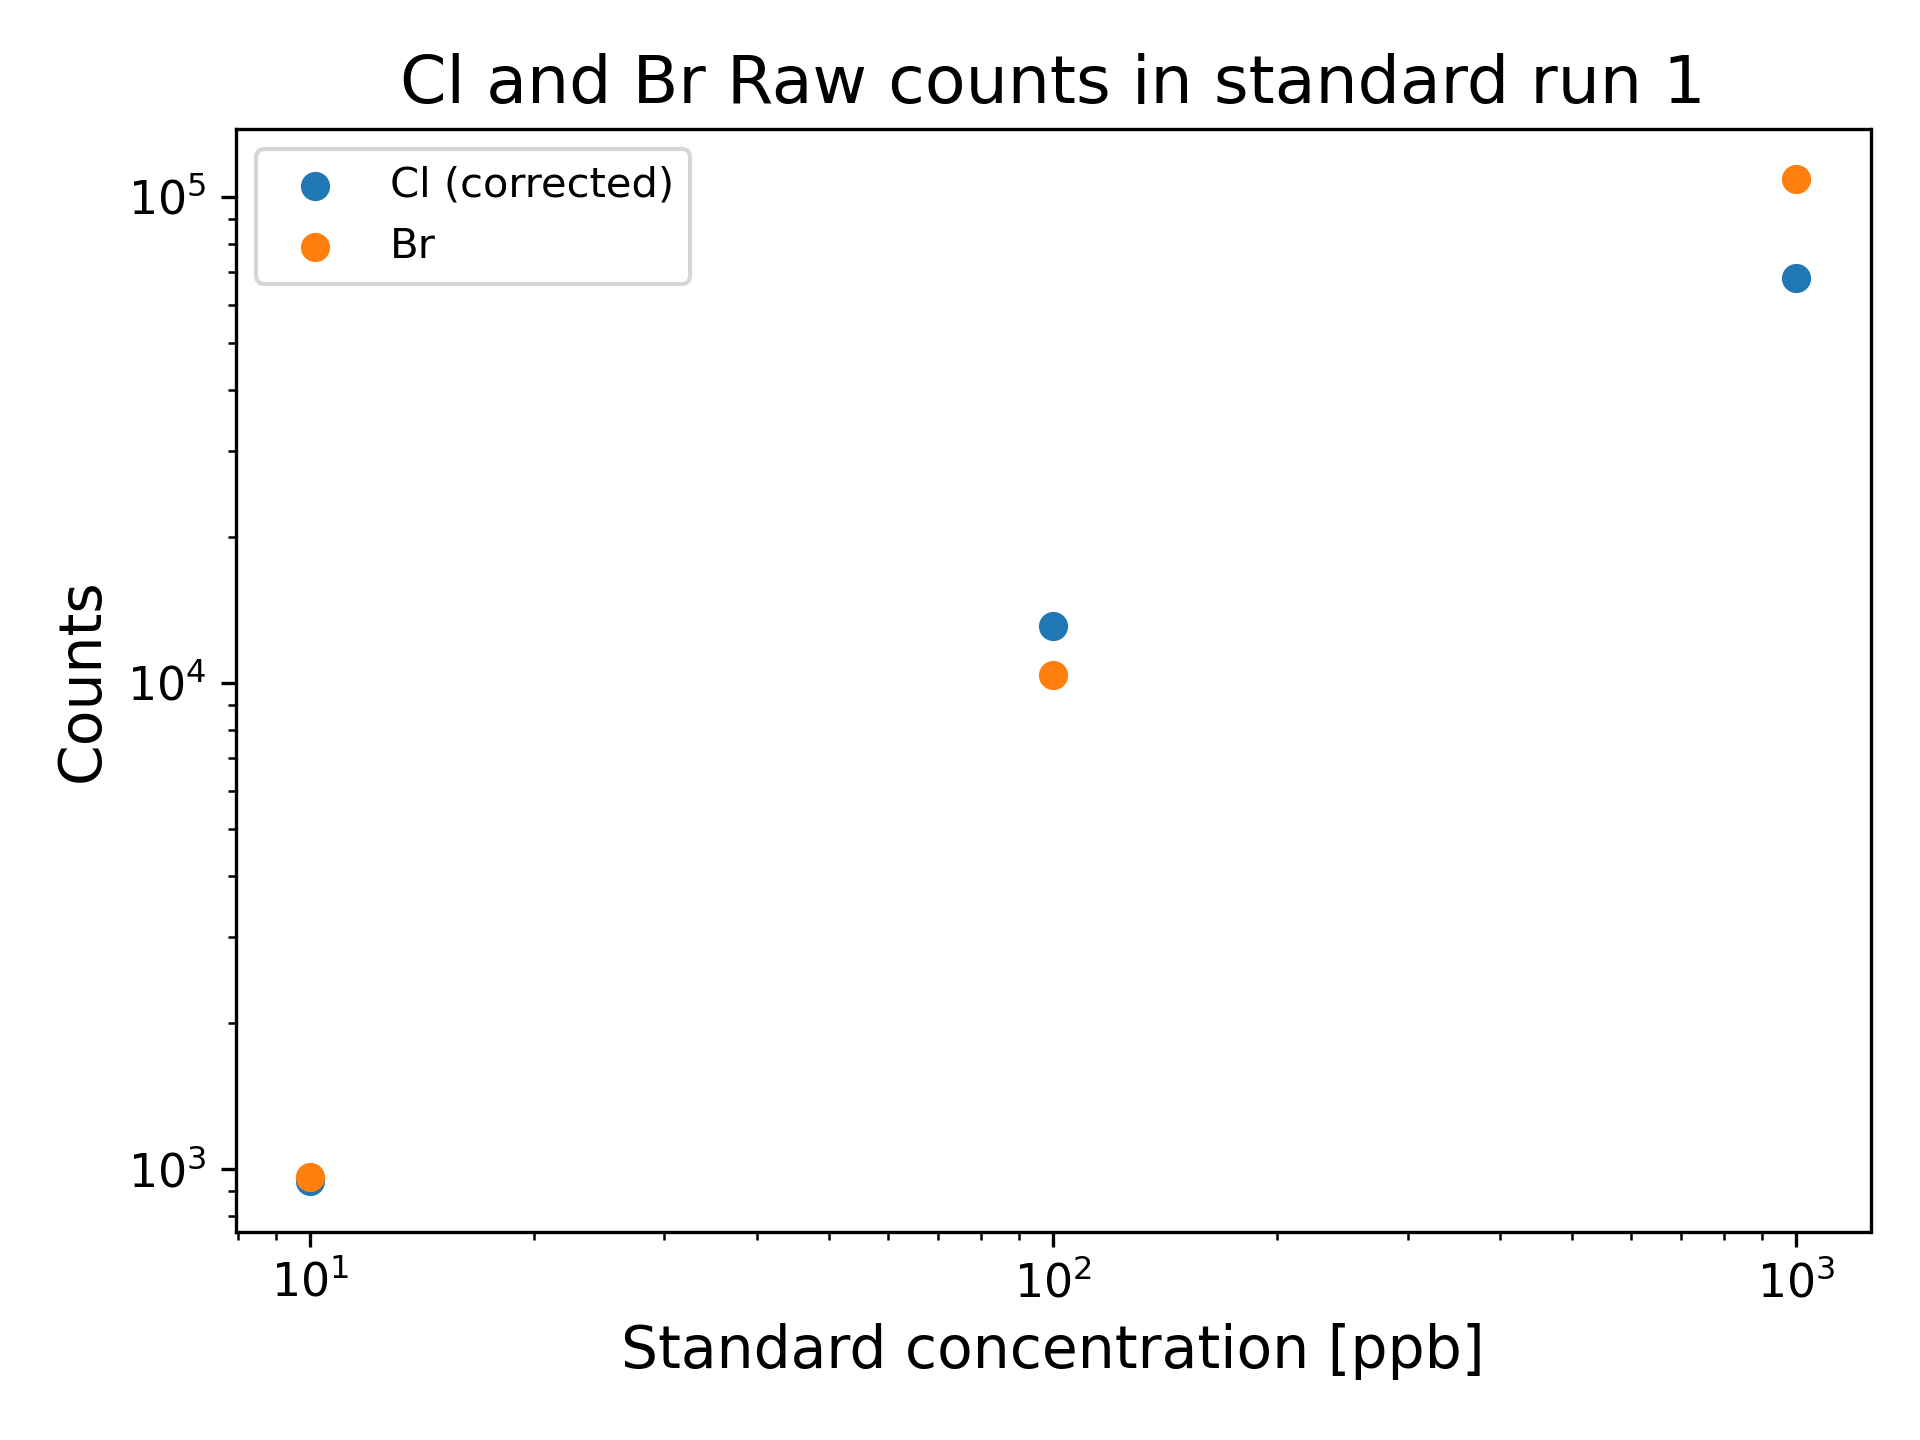
\includegraphics[width=0.45\textwidth]{img/cl_br_standards_run1.png}}\qquad
    \subfigure[Standard Cl and Br counts \emph{after} measuring samples.\label{fig:cl-br-counts-run3}]{
        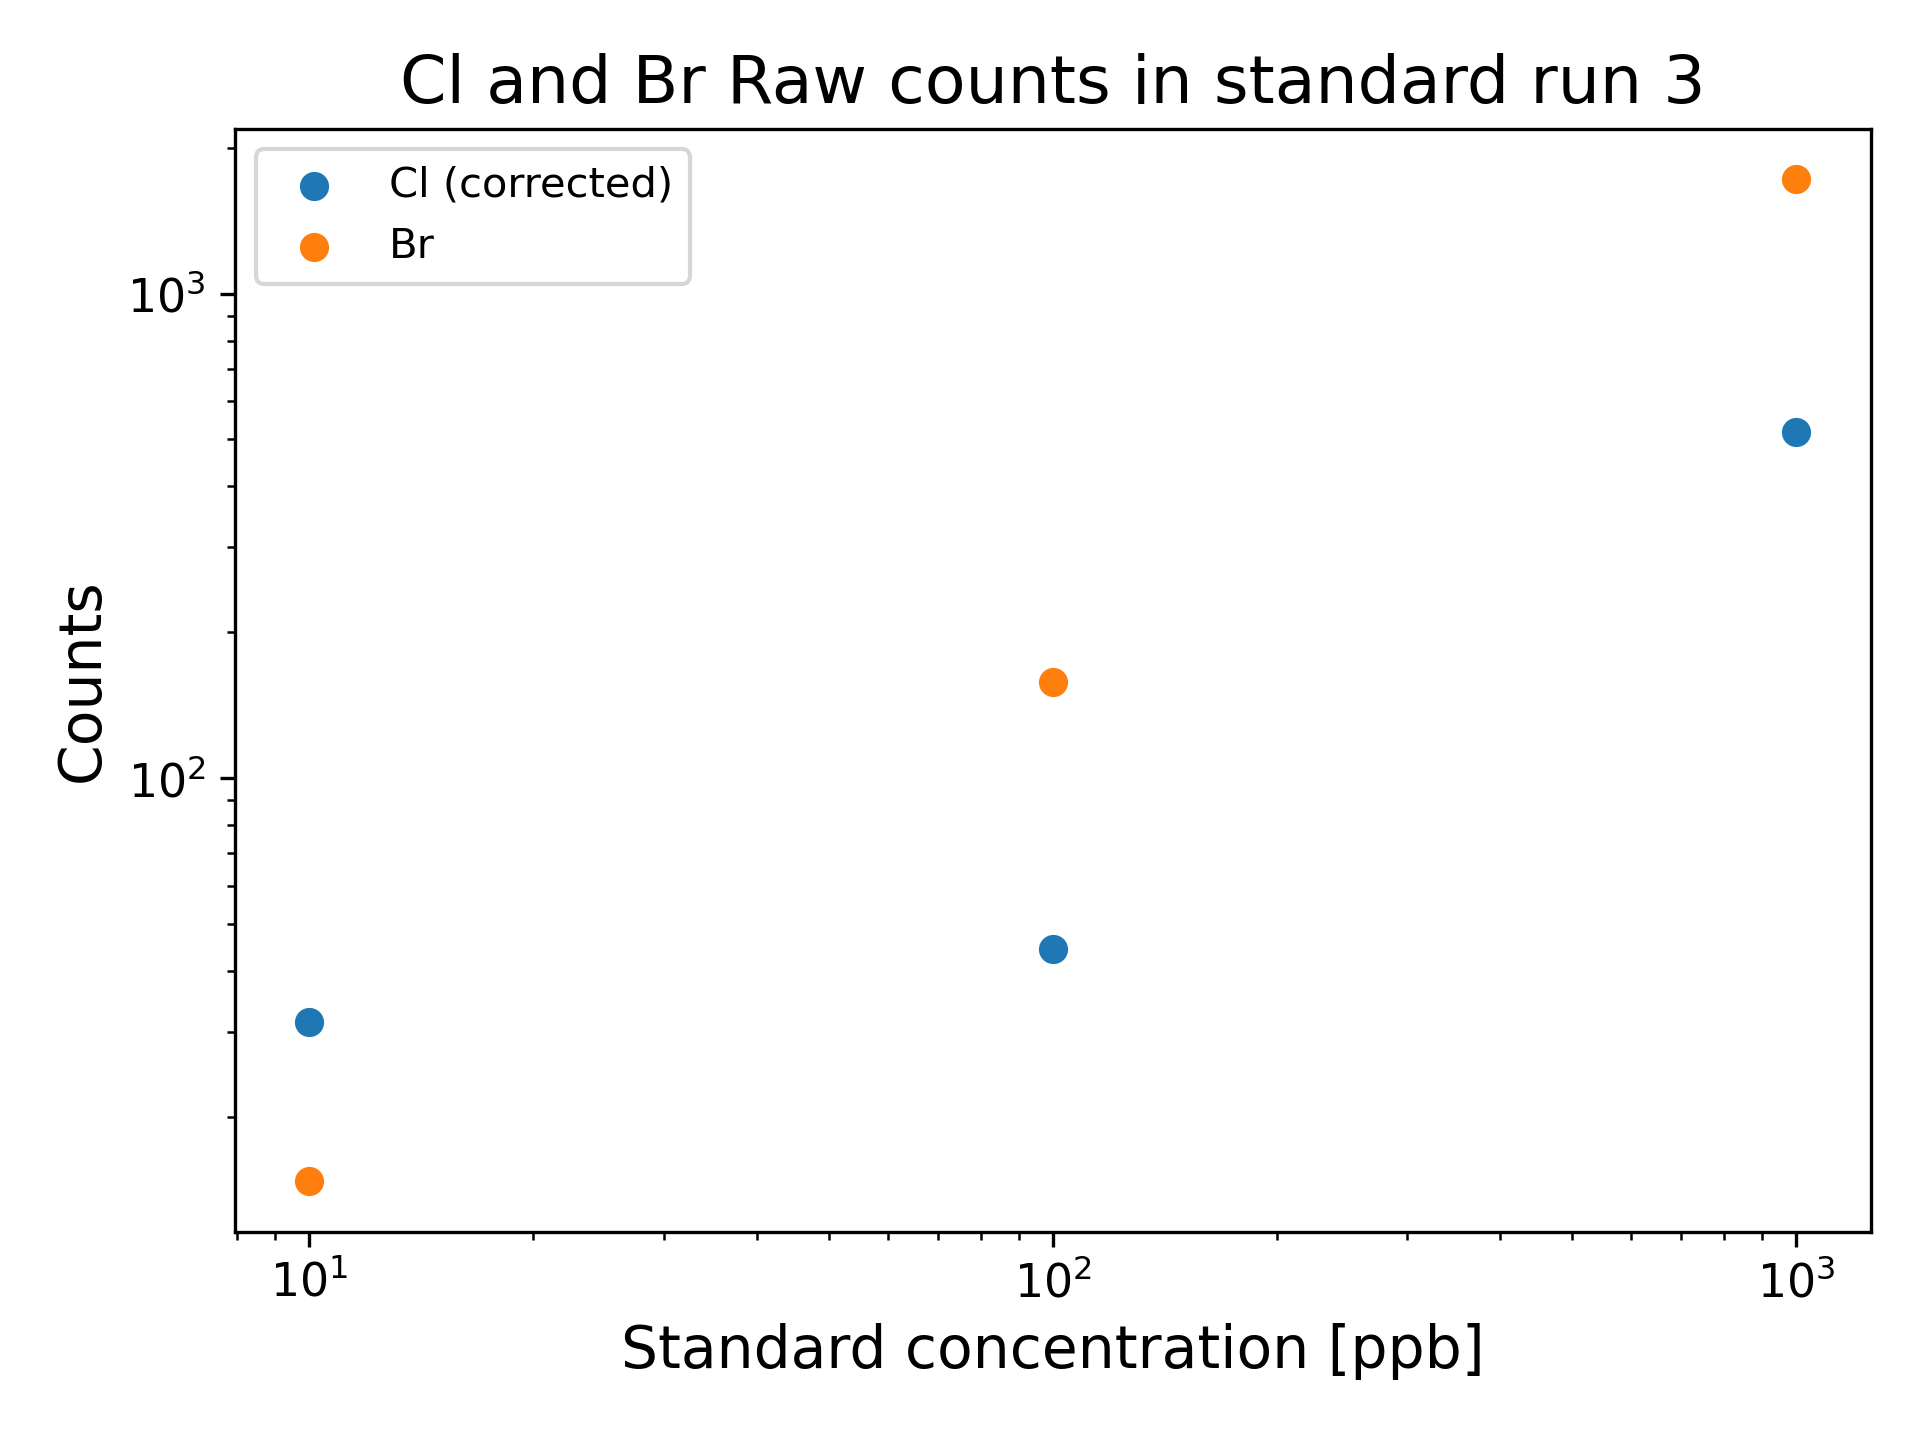
\includegraphics[width=0.45\textwidth]{img/cl_br_standards_run3.png}}
    \caption{Cl (after correction) and Br show the expected linear dependence on
    solution concentrations at the beginning of the measurement (run 1), but
    Cl is not linear in the final run 3.}
    \label{fig:cl-br-counts}
\end{figure}

\textcite{wei-2020} determined Sr/Ba ratios of 0.5 and 0.2 as thresholds between marine/brackish and 
brackish/freshwater. These ratios are plotted as light grey lines. Third, the ROC curve best fit ratio
is plotted the red lines. The best fit lines are corrected for the outlier JWL 1. 
The plots for both measurement methods show that the data do not fit the model from \textcite{wei-2020}.

\section{S/TOC}

\acro{IRMS} yielded \TOC measurements for all samples, but no uncertainties were determined.
\XRF and \ICPMS consistently measured \acro{S} for all samples~(\cref{tab:s-toc-table,tab:s-toc-icpms-table}).
For XRF, we obtained results for two pellets for each sample and standard, whereas only one \TOC result
was available for each. Therefore, to match measurements for S from XRF with \TOC, we averaged the S results
of the two pellets per sample.

\Cref{fig:toc_s_crossplot} shows cross-plots of \acro{S} over \TOC. The plot layout is 
similar to that for Sr/Ba (\cref{fig:sr_ba_crossplot}), but the brackish/freshwater threshold is 
0.1 instead of 0.2. Additionally, it shows the normal trend for S/TOC in marine settings
from \textcite{berner-raiswell-1983}. The normal freshwater trend, also proposed by these authors, coincides 
with the brackish threshold of \textcite{wei-2020}, therefore it is not plotted separately.

\begin{figure}
    \centering
    \includegraphics*[width=0.95\textwidth]{img/sr_ba_combined.png}
    \caption{Sr/Ba data from XRF (left) and \ICPMS (right). 
    The colour coding into marine (UMM/Flysch) and freshwater (USM/OSM) is
    based on the classification of the sample locations in \textcite{Linth_Map}. 
    The grey lines are the dividers given by \textcite{wei-2020},
    the red line is a best fit for our data.
    }\label{fig:sr_ba_crossplot}    
\end{figure}

The most notable difference between the \XRF and \ICPMS data is the \acro{S} concentration for 
marine samples.
\ICPMS reported concentrations approximately twice as high as those from \XRF, 
while the freshwater samples showed roughly the same concentrations
with both methods. Because \TOC was determined independently and only once,
the x-axis is identical in both plots. 

Despite the differences, both datasets show that marine and freshwater samples group in two 
distinct clusters.
The freshwater samples fall 
into the freshwater sector proposed by \textcite{wei-2020} and close to the general
freshwater trend of \textcite{berner-raiswell-1983}. The marine samples fall
into the brackish sector, and in the case of the \XRF data, much closer to the freshwater trend 
than to the marine trend of \textcite{berner-raiswell-1983}. JWL 1 is an exception in all cases
and shows a strong marine signal.

With the XRF data, the fitted threshold falls below the normal freshwater trend
from \textcite{berner-raiswell-1983}, and all data points are close to that threshold. 
With \ICPMS, the fitted threshold falls between the marine and freshwater
trends.


\section{Carbonate}

Carbonates can influence the Sr content in sedimentary rocks significantly~\parencite{wei-2020}.
To estimate the upper bound on carbonate content in our samples, we attributed all Ca (measured with \ICPMS)
to CaCO$_3$ (\cref{fig:carbonate}). 

This estimate is reasonable, because the main Ca-bearing minerals in rocks are carbonates,
feldspars, pyroxenes and evaporites. In fine-grained detrital sediments in marginal settings, like those in our 
case study, most of these minerals have undergone chemical weathering and are either fully dissolved or
have been altered to clays, which contain little Ca in their crystal structure. Ca may adsorb to
clays, which is why our estimates represent upper bounds to carbonate.

\begin{figure}
    \centering
    \includegraphics*[width=0.95\textwidth]{img/toc_s_combined.png}
    \caption{S data from XRF(left) and \ICPMS(right), TOC from IRMS. 
    The colour coding into marine (UMM/Flysch) and freshwater (USM/OSM) is
    based on the classification of the sample locations in \textcite{Linth_Map}. 
    The light grey lines are the dividers given by \textcite{wei-2020}, the dark grey line
    is the normal marine trend for S/TOC from
    \textcite{berner-raiswell-1983}, the red line is a best fit for our data.
    }\label{fig:toc_s_crossplot}    
\end{figure}

\begin{figure}[b]
    \centering
    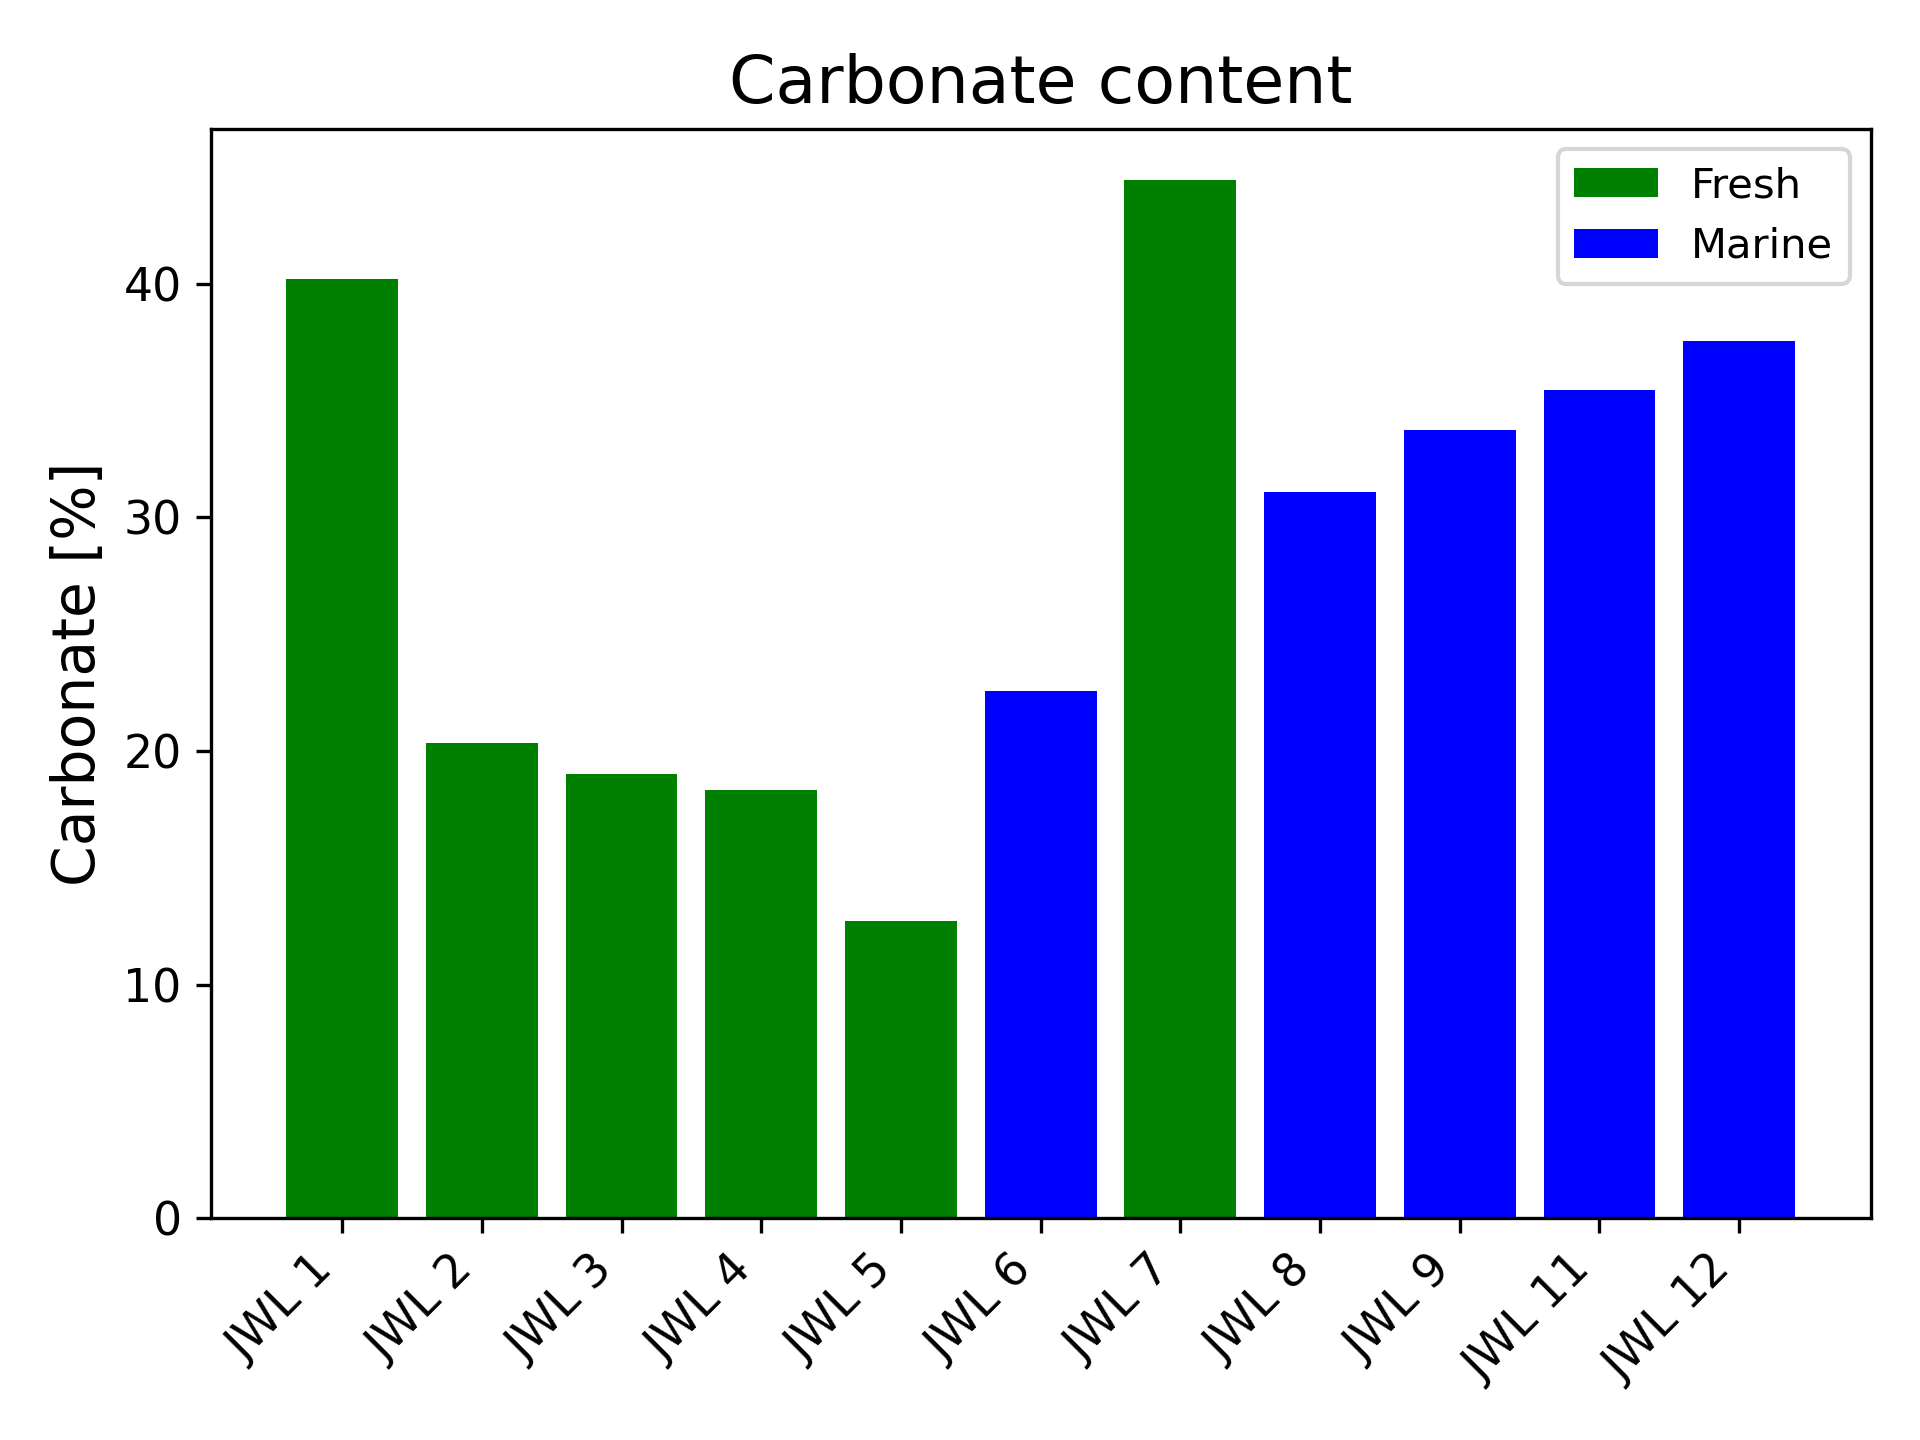
\includegraphics[width=.4\textwidth]{img/icpms_carbonate.png}
    \caption{Upper bounds on carbonate content in the samples estimated from Ca measurements with \ICPMS,
    attributing all measured Ca to CaCO$_3$.}
    \label{fig:carbonate}
\end{figure}
\chapter{Discussion}

A good proxy for depositional environments must show a strong correlation to
the environments and should be insensitive to confounding influences.
Salinity would be a good proxy, because it differs substantially between freshwater, brackish and marine 
conditions, and few environments other than oceans show high salinity. However,
the salinity of their formation waters is often not preserved reliably in sediments \parencite{kharaka-2003}.
The (trace) element ratios we discuss here have been proposed in the literature as proxies
for \emph{salinity}, and thus indirectly indicate marine, brackish 
and freshwater conditions.

\section{Data quality}

Uncertainties in our measurements stem from two sources: sample preparation and analytical procedures,
and the statistical uncertainty of the measurement methods. Uncertainties due
to sample preparation and analytical procedures cannot be measured and remain unknown in most cases.
Only the \XRF instrument reports the Compton ratio as an indication whether the quality of the sample allows
reproducible measurements. 
Both, the \XRF and \ICPMS instruments report the statistical uncertainty of measurements (\cref{tab:sr-ba-table,tab:sr-ba-icpms-table,tab:s-toc-icpms-table}).

The concentrations reported by \XRF and \ICPMS differ substantially. 
\XRF reported about twice the concentrations of \acro{Ba}, and half the concentration of \acro{S}.
Because the statistical uncertainty was roughly 10\% for S and Ba for both methods, the large difference
must stem from sample preparation and analytical procedures.
While the \ICPMS method with HF digestion is known to produce reliable results,
the \XRF instrument is new, uncalibrated, was used without standards, and reported moderate to poor 
Compton ratios.
This suggests that the large discrepancy between the two methods was caused by the
uncalibrated and thus unreliable \XRF method. Therefore, the following discussion focusses
only on the \ICPMS results and skips the \XRF results.

The ROC-based best-fit algorithm combined with Youden's J statistic has limitations. 
It is an approximation that
requires that the resulting straight line always passes through at least one of the observed data points. 
When the data forms tight, well separated clusters, the derived fitting line could be far from the optimum.
This deviation from the theoretical optimum does not affect the classification of the fitted samples, 
but generalizing the result to other samples needs to be approached cautiously.

\section{Sr/Ba}

Strontium and Barium are both alkaline-earth elements.
The radius of the Sr atom is slightly larger than that of \acro{Ca}, 1.26\,\AA\ vs. 1\,\AA, and slightly smaller 
than potassium (\acro{K}, 1.38\,\AA). Sr can
substitute for \acro{Ca} and the monovalent \acro{K} in some minerals. The radius 
of \acro{Ba} (1.42\,\AA) is too large to substitute
for \acro{Ca} in most crystal lattices, particularly in calcite~\parencite{housecroft-chemistry}.
Under chemical weathering Sr preferentially leaves the crystal lattice. It is
mobile, leading to higher Sr concentrations in the oceans compared to freshwater~\parencite{brand-veizer-1980}.
The main sink for Sr in the oceans is substitution for Ca in biogenic carbonates, and in brines with high Sr concentrations,
the formation of strontianite (SrCO$_3$)~\parencite{banner-hanson-1990,wei-2020}.

Ba in silicate minerals weathers less readily than Sr, the main Ba weathering flux comes from barite (BaSO$_4$)
and witherite (BaCO$_3$)~\parencite{wei-2020}.
Due to the very low solubility of its sulphates and sulphides, Ba is not mobile and occurs only in very low 
concentrations in all waters. In freshwater, Ba is transported primarily 
adsorbed to clay minerals. With increasing salinity, ion exchange desorbs Ba from the clays~\parencite{wei-2020}.
Most Ba in the oceans precipitates as
barite (BaSO$_4$) due to the high concentration of SO$_{4}^{2-}$ in the oceans.

The data in \cref{fig:sr_ba_crossplot} are not clearly
separated into marine and freshwater sectors, and the thresholds for the \acro{Sr}/\acro{Ba}
ratios proposed by \textcite{wei-2020} fit our samples poorly~(cf. \cref{tab:icpms-classification}).
The misfit between our data and the model from \textcite{wei-2020} is caused by our \acro{Sr} values being
considerably
higher than the mean values from \textcite{wei-2020} (\cref{fig:sr-ba-wei}). There are several possible
explanations for this. 

\begin{table}[b!]
    \centering
    \caption{Classification of our samples into marine (M), brackish (B) and freshwater (F) according to different methods.
    Where applicable we compare our data against the classification criteria of \textcite{wei-2020}. 
    Geological map classification based on \textcite{Linth_Map}.}\label{tab:icpms-classification}
    \input{temp/icpms-classification-table.txt}
\end{table}

% First, \cref{fig:sr-ba-wei} shows that there are some outliers of marine sediments with high \acro{Sr}
% values in the dataset from \textcite{wei-2020}, and the case study discussed in detail by them
% concludes that the samples have abnormally high Sr values without an explanation. 
% Therefore, it is possible that our samples simply have
% abnormally high \acro{Sr} values that the global model cannot explain. 

First, it is possible that the rocks that we classified as freshwater sediments are
actually sediments from brackish or marine environments.
However, the S/TOC data discussed in the next section contradicts this interpretation.

Second, \textcite{wei-2020} state that
carbonate-rich rocks may have high concentrations of \acro{Sr}, because \acro{Sr} can substitute
for \acro{Ca} in calcite (up to 10\,000\,ppm) and aragonite (up to 80\,000\,ppm).
However, such high concentrations are only observed in biogenic carbonates and calcite recrystallized from aragonite, 
but not carbonates precipitated from solution (Picotti, V., 05/2026, personal communications). Mud-
and siltstones contain carbonates only as cement, which is precipitated, not biogenic. 

\textcite{banner-hanson-1990}
developed a theoretical model to estimate the equilibrium concentrations of Sr between precipitated calcite and water.
As an example, in solutions with 10\,ppm Sr, the equilibrium concentration in calcite is 200\,ppm. 
Given typical concentrations of Sr in natural waters (mean 40\,ppb in freshwater and 8\,ppm in seawater)
\parencite{musgrove-2021,wei-2020}, the model predicts Sr concentrations below 200\,ppm in carbonates.
Our measured concentrations are much higher than 200\,ppm.
Considering that the carbonate content in our
samples is only 13--44\%, carbonates with an expected Sr concentration less than 200\,ppm cannot 
be the only explanation for the high Sr concentrations.

\begin{figure}
    \centering
    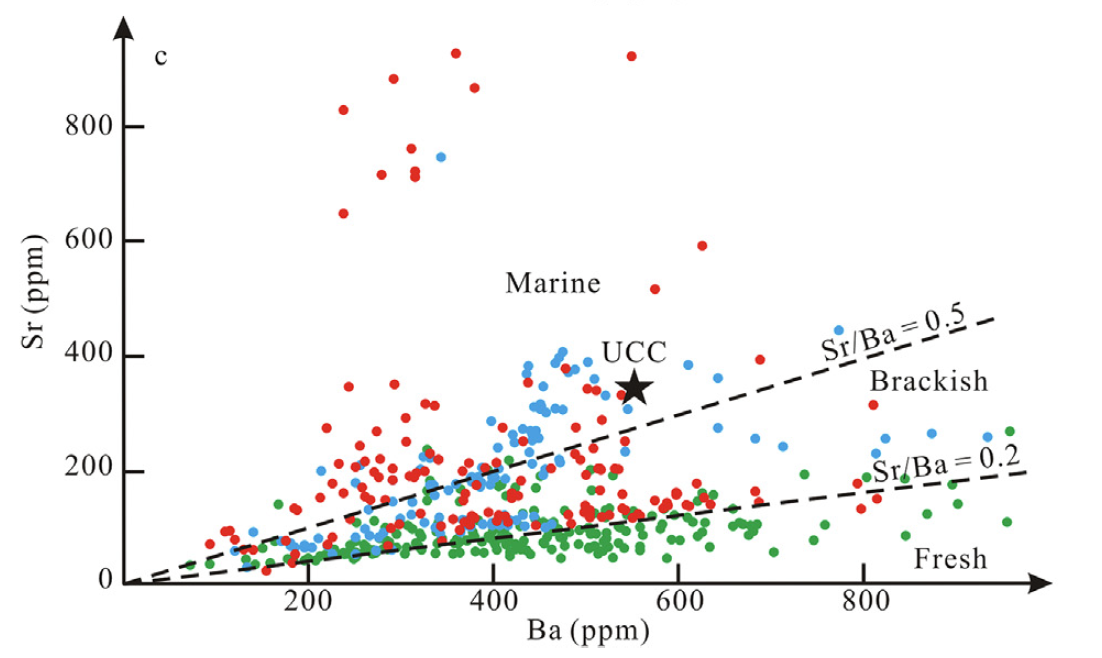
\includegraphics[width=0.5\textwidth]{img/sr-ba-wei.png}
    \caption{Sr/Ba cross-plot of all data from \textcite{wei-2020}. The mean Sr value is approximately 200\,ppm.
    Colour coding: freshwater green, brackish blue, marine red.}
    \label{fig:sr-ba-wei}
\end{figure}

\begin{figure}
    \centering
    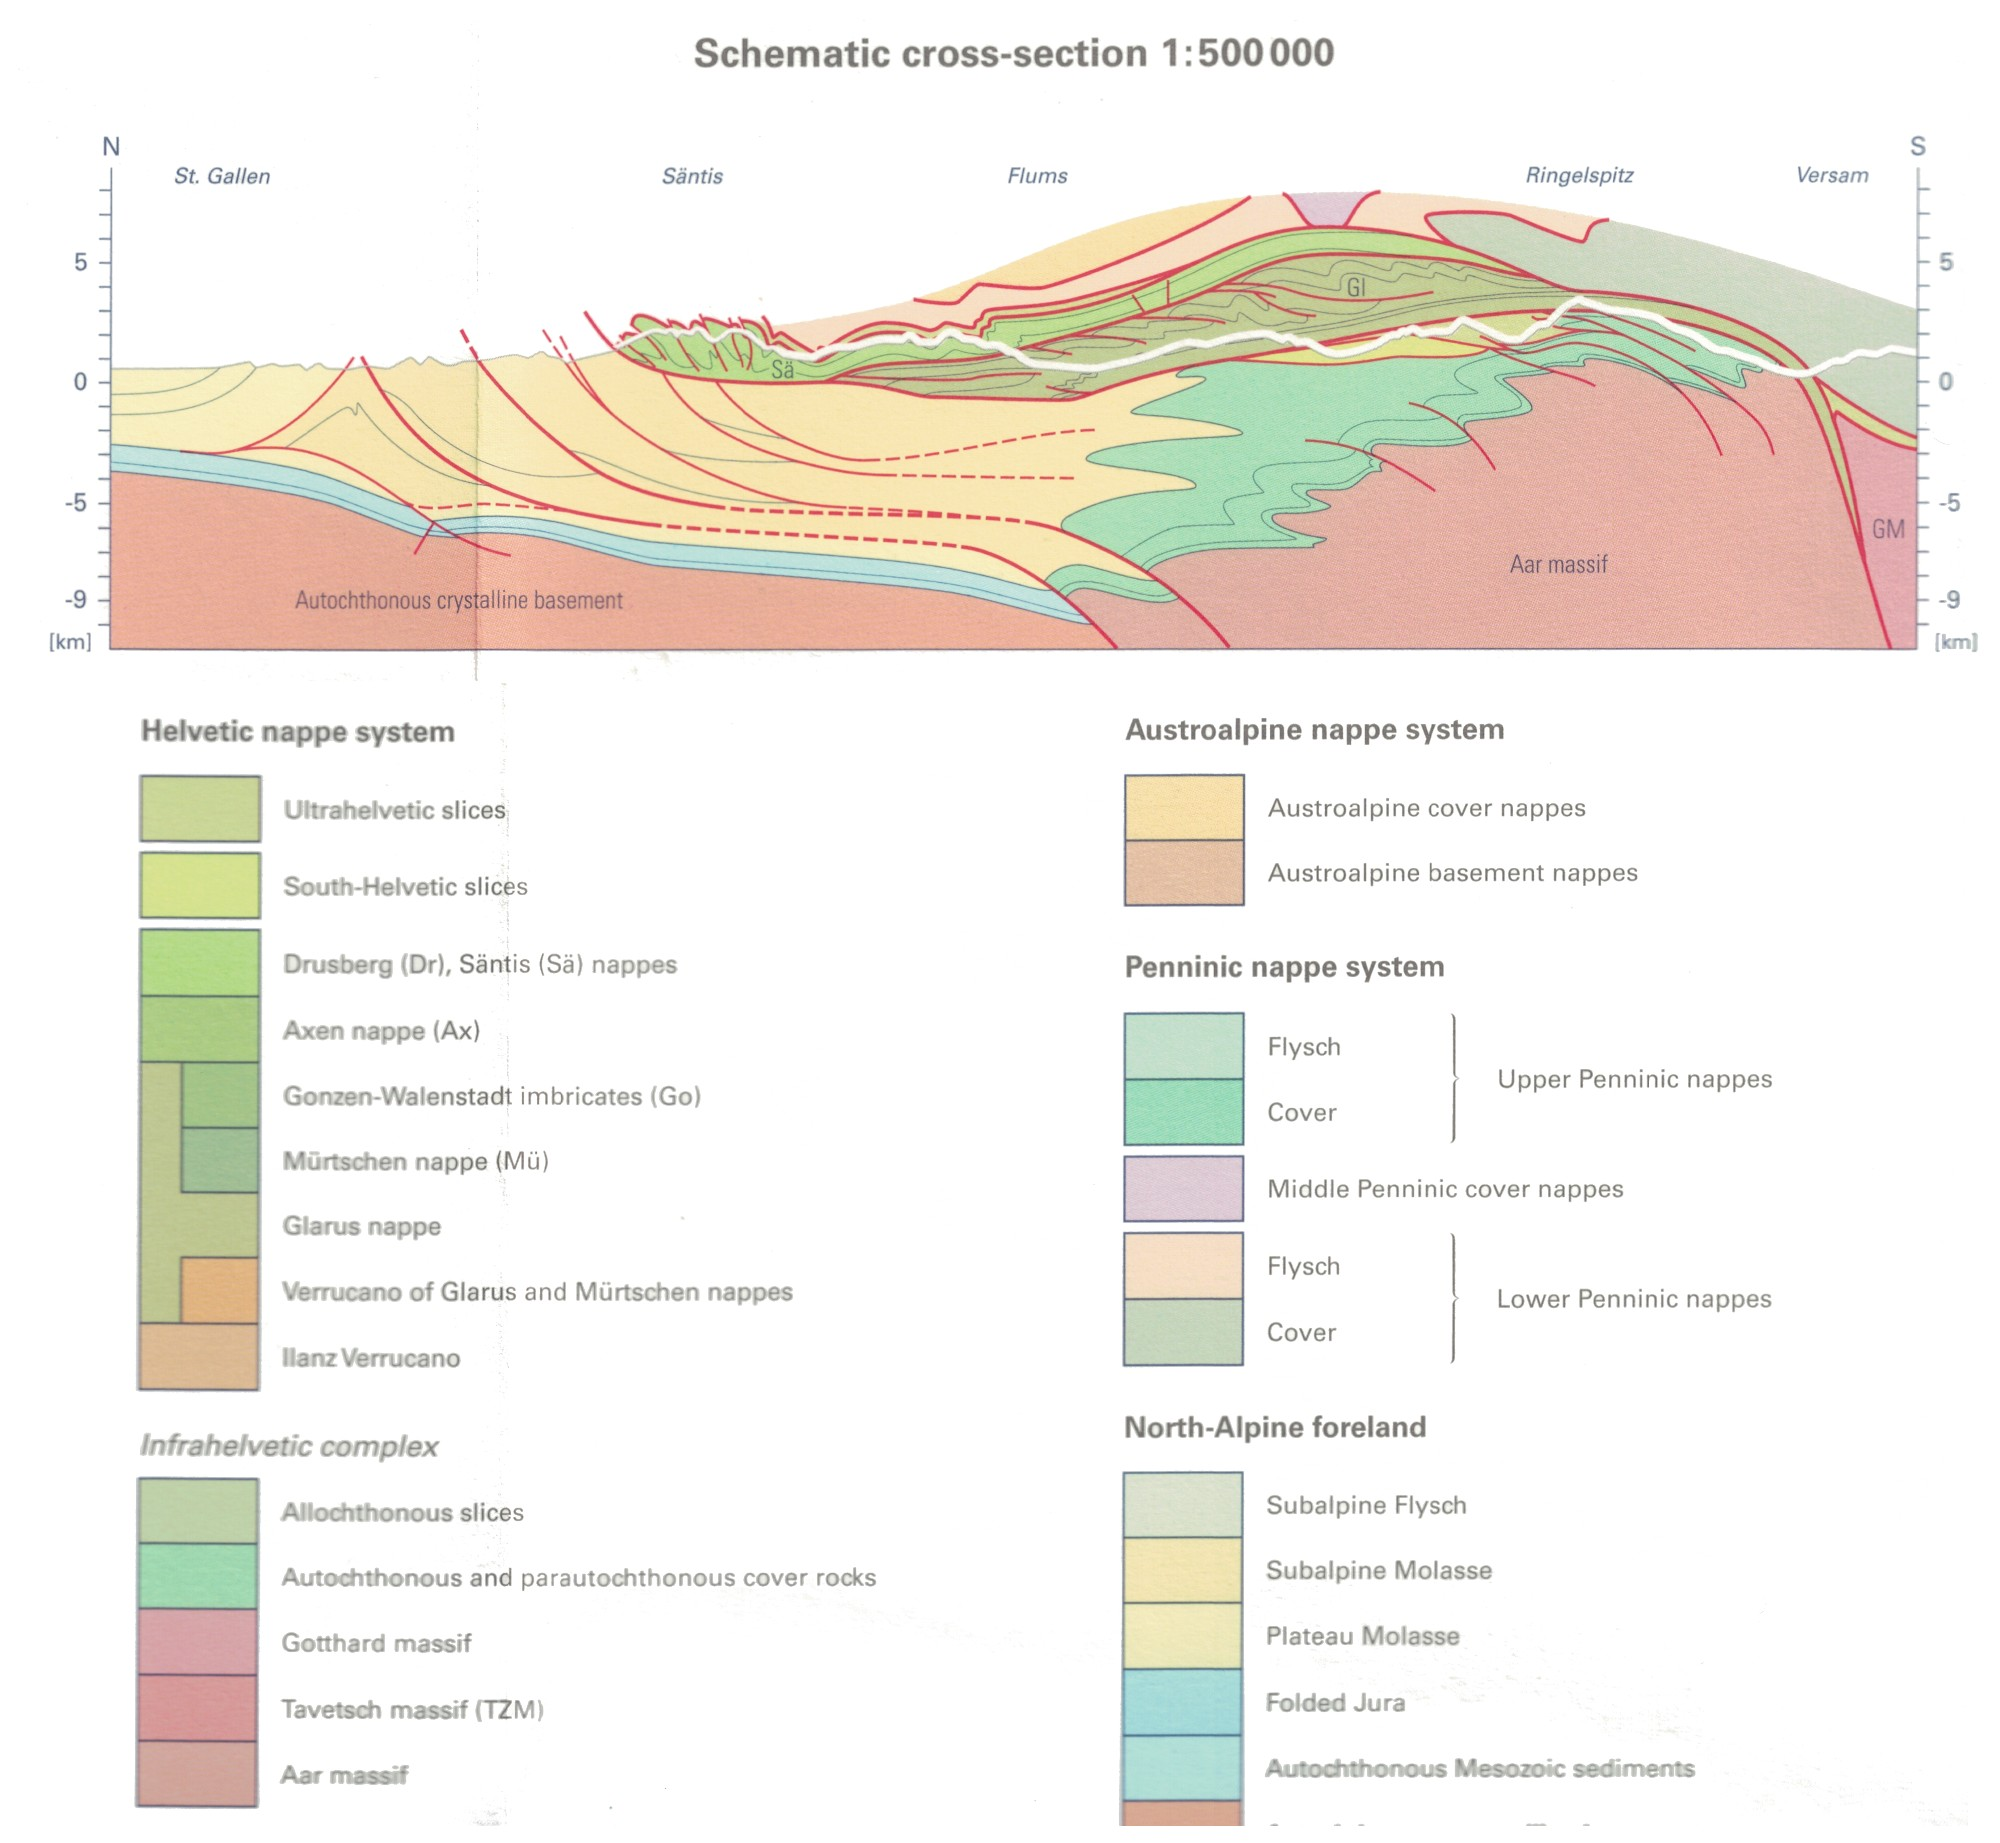
\includegraphics[width=.95\textwidth]{img/profile_large.jpg}
    \caption{Schematic cross-section through the SMB and subalpine molasse in the study area. The 
    subalpine molasse originally rests on the Mesozoic sediments, and potentially early Cenozoic
    sediments. The study area lies at the surface contact between the Subalpine Molasse and overthrust
    Helvetic nappe. Source: \textcite[map sheet 33]{helvetic-map}}
    \label{fig:overview-profile}
\end{figure}

Third, \textcite{kharaka-2003} studied deep water
bodies, which typically have very high amounts of \TDS. They found that
\acro{Sr} concentrations correlate strongly with \TDS and can reach several hundred ppm in
those deep brines. These high \TDS values usually occur in aquifers that are in contact with
limestone and/or evaporites like gypsum and anhydride.

The \UMM was deposited on top of the Mesozoic sediments that underlie the entire \SMB 
(\cref{fig:overview-profile}, \textcite{helvetic-map}). Locally, the \UMM may lie on the
marls of the late Eocene Stad and Euthal formations \parencite{Ibergeregg_Text}, but in Eastern
Switzerland, the molasse usually rests on the Jurassic Malm limestones \parencite{chevalier-molasse-2010}.
The Stad and Euthal formations are rich in fossils \parencite{Einsiedeln_Text}, 
and the upper Malm limestones represent a carbonate platform \parencite{chevalier-molasse-2010}, 
so they may contain very high concentrations of 
\acro{Sr}. When these sediments were buried under the UMM, compaction may have expelled the briny pore waters,
which then would have risen upwards and transported the contained Sr into the UMM sediments, where they
provided the high
Sr concentrations in the pore waters from which the calcite cement precipitated~\parencite{kharaka-2003}.

% \begin{table}
%     \centering
%     \caption{Classification of our rocks samples into marine (M), brackish (B) and freshwater (F) according to different methods.
%     Where applicable we compare our data against the classification criteria of \textcite{wei-2020}. 
%     Geological map classification based on \textcite{Linth_Map}.}\label{tab:xrf-classification}
%     \input{temp/xrf-classification-table.txt}
% \end{table}

Overall, our data suggest that without calibration to local conditions, e.g. by using a few standard samples
of known origin to define the classification threshold, the Sr/Ba ratio cannot be used reliably for the classification
into marine/freshwater conditions. 

\section{S/TOC}

Sulphur occurs in many minerals and is a major constituent of organic matter.
In aqueous solution S usually exists in the oxidized form of sulphate (SO$_4^{2-}$), which is
highly mobile and is transported to the oceans. The average sulphate concentrations are
27\,ppm in freshwater and 2900\,ppm in seawater \parencite{wei-2020}.
This difference in concentration is reflected in the amount of S preserved in sediments.

The preservation of \acro{S} and organic carbon in sediments is mainly controlled by 
bacterial sulphate reduction in anoxic sediments rich in organic matter~\parencite{berner-raiswell-1983}.
During this process, sulphate is reduced to sulphide and organic matter is destroyed. 
The sulphide and the surviving organic matter are deposited as metal sulphides and \TOC, respectively.
\textcite{berner-raiswell-1983} estimate the S/TOC ratio in marine sediments to be around 0.33 and
in freshwater 0.1 or even less. These trends are shown as dark grey lines in \cref{fig:toc_s_crossplot}.

Our data forms well separated clusters and fits the model by \textcite{wei-2020} 
reasonably well~(\cref{fig:toc_s_crossplot}), again except for sample JWL 1.
The best fit line lies in the middle of the brackish sector from \textcite{wei-2020}, 
and between the general trends proposed by \textcite{berner-raiswell-1983}. 
Overall, the S/TOC ratio separates marine and freshwater sediments
clearly and appears to be suitable for classification, even
without local calibration.

\section{A marine transgression?}

Sample JWL 1, a USM sample according to \textcite{Linth_Map}, was classified as marine
by all methods and thresholds from the literature as well as our best fit 
thresholds~(\cref{tab:icpms-classification}). 
It exhibits a much higher S/TOC ratio than all other samples. 
While it is possible for such an S/TOC ratio to occur in lake sediments with euxinic conditions 
in the water column, such lakes are rare \parencite{berner-raiswell-1983}. It is 
far more likely that the high S/TOC is a strong marine signal.

All marine samples contain
significantly more carbonate than freshwater samples. The exception are our two reference
samples for flysch (JWL 6) and \OSM (JWL 7), where the order is reversed (\cref{fig:carbonate}).
This is consistent with their depositional settings:
flysch is a detrital deep marine sediment, less likely to contain carbonate, and the \OSM is known to contain 
a lot of freshwater carbonate (e.g. \parencite{gubler_2009e}). The climate also differed 
between the Eocene flysch and the late Miocene \OSM deposition,
which likely influenced the overall chemistry of the sediments \parencite{schlunegger_possible_2007}.
JWL~1 has the second-highest carbonate content of all samples, which supports its interpretation as a 
marine sediment.

JWL~1--3 were collected from the same \USM outcrop (\cref{fig:log_L1}).
Our measurements confirm that JWL~2 and 3 are freshwater sediments, and suggest that JWL~1 is a marine sediment.
Whether this represents a period of marine transgression or whether this layer was folded in between the
freshwater sediments during the period of strong tectonic deformation of the subalpine molasse
is a question we cannot answer with the geochemical data obtained in this study.

The mudrocks above the gap in the outcrop (\cref{fig:log_L1}), 
especially the bed in directly below the overlying sandstone,
show fractures and slickensides indicating fault movement. 
This raises questions about the nature of the unexposed interval. 
It is more weathered and overgrown: is that because the rock is more fractured, 
like a fault gouge, or is it made of softer, more easily weathered sediments than the surrounding
outcrop? Indications of where exactly the change in depositional environment happened may be buried there.

\begin{figure}
    \centering
    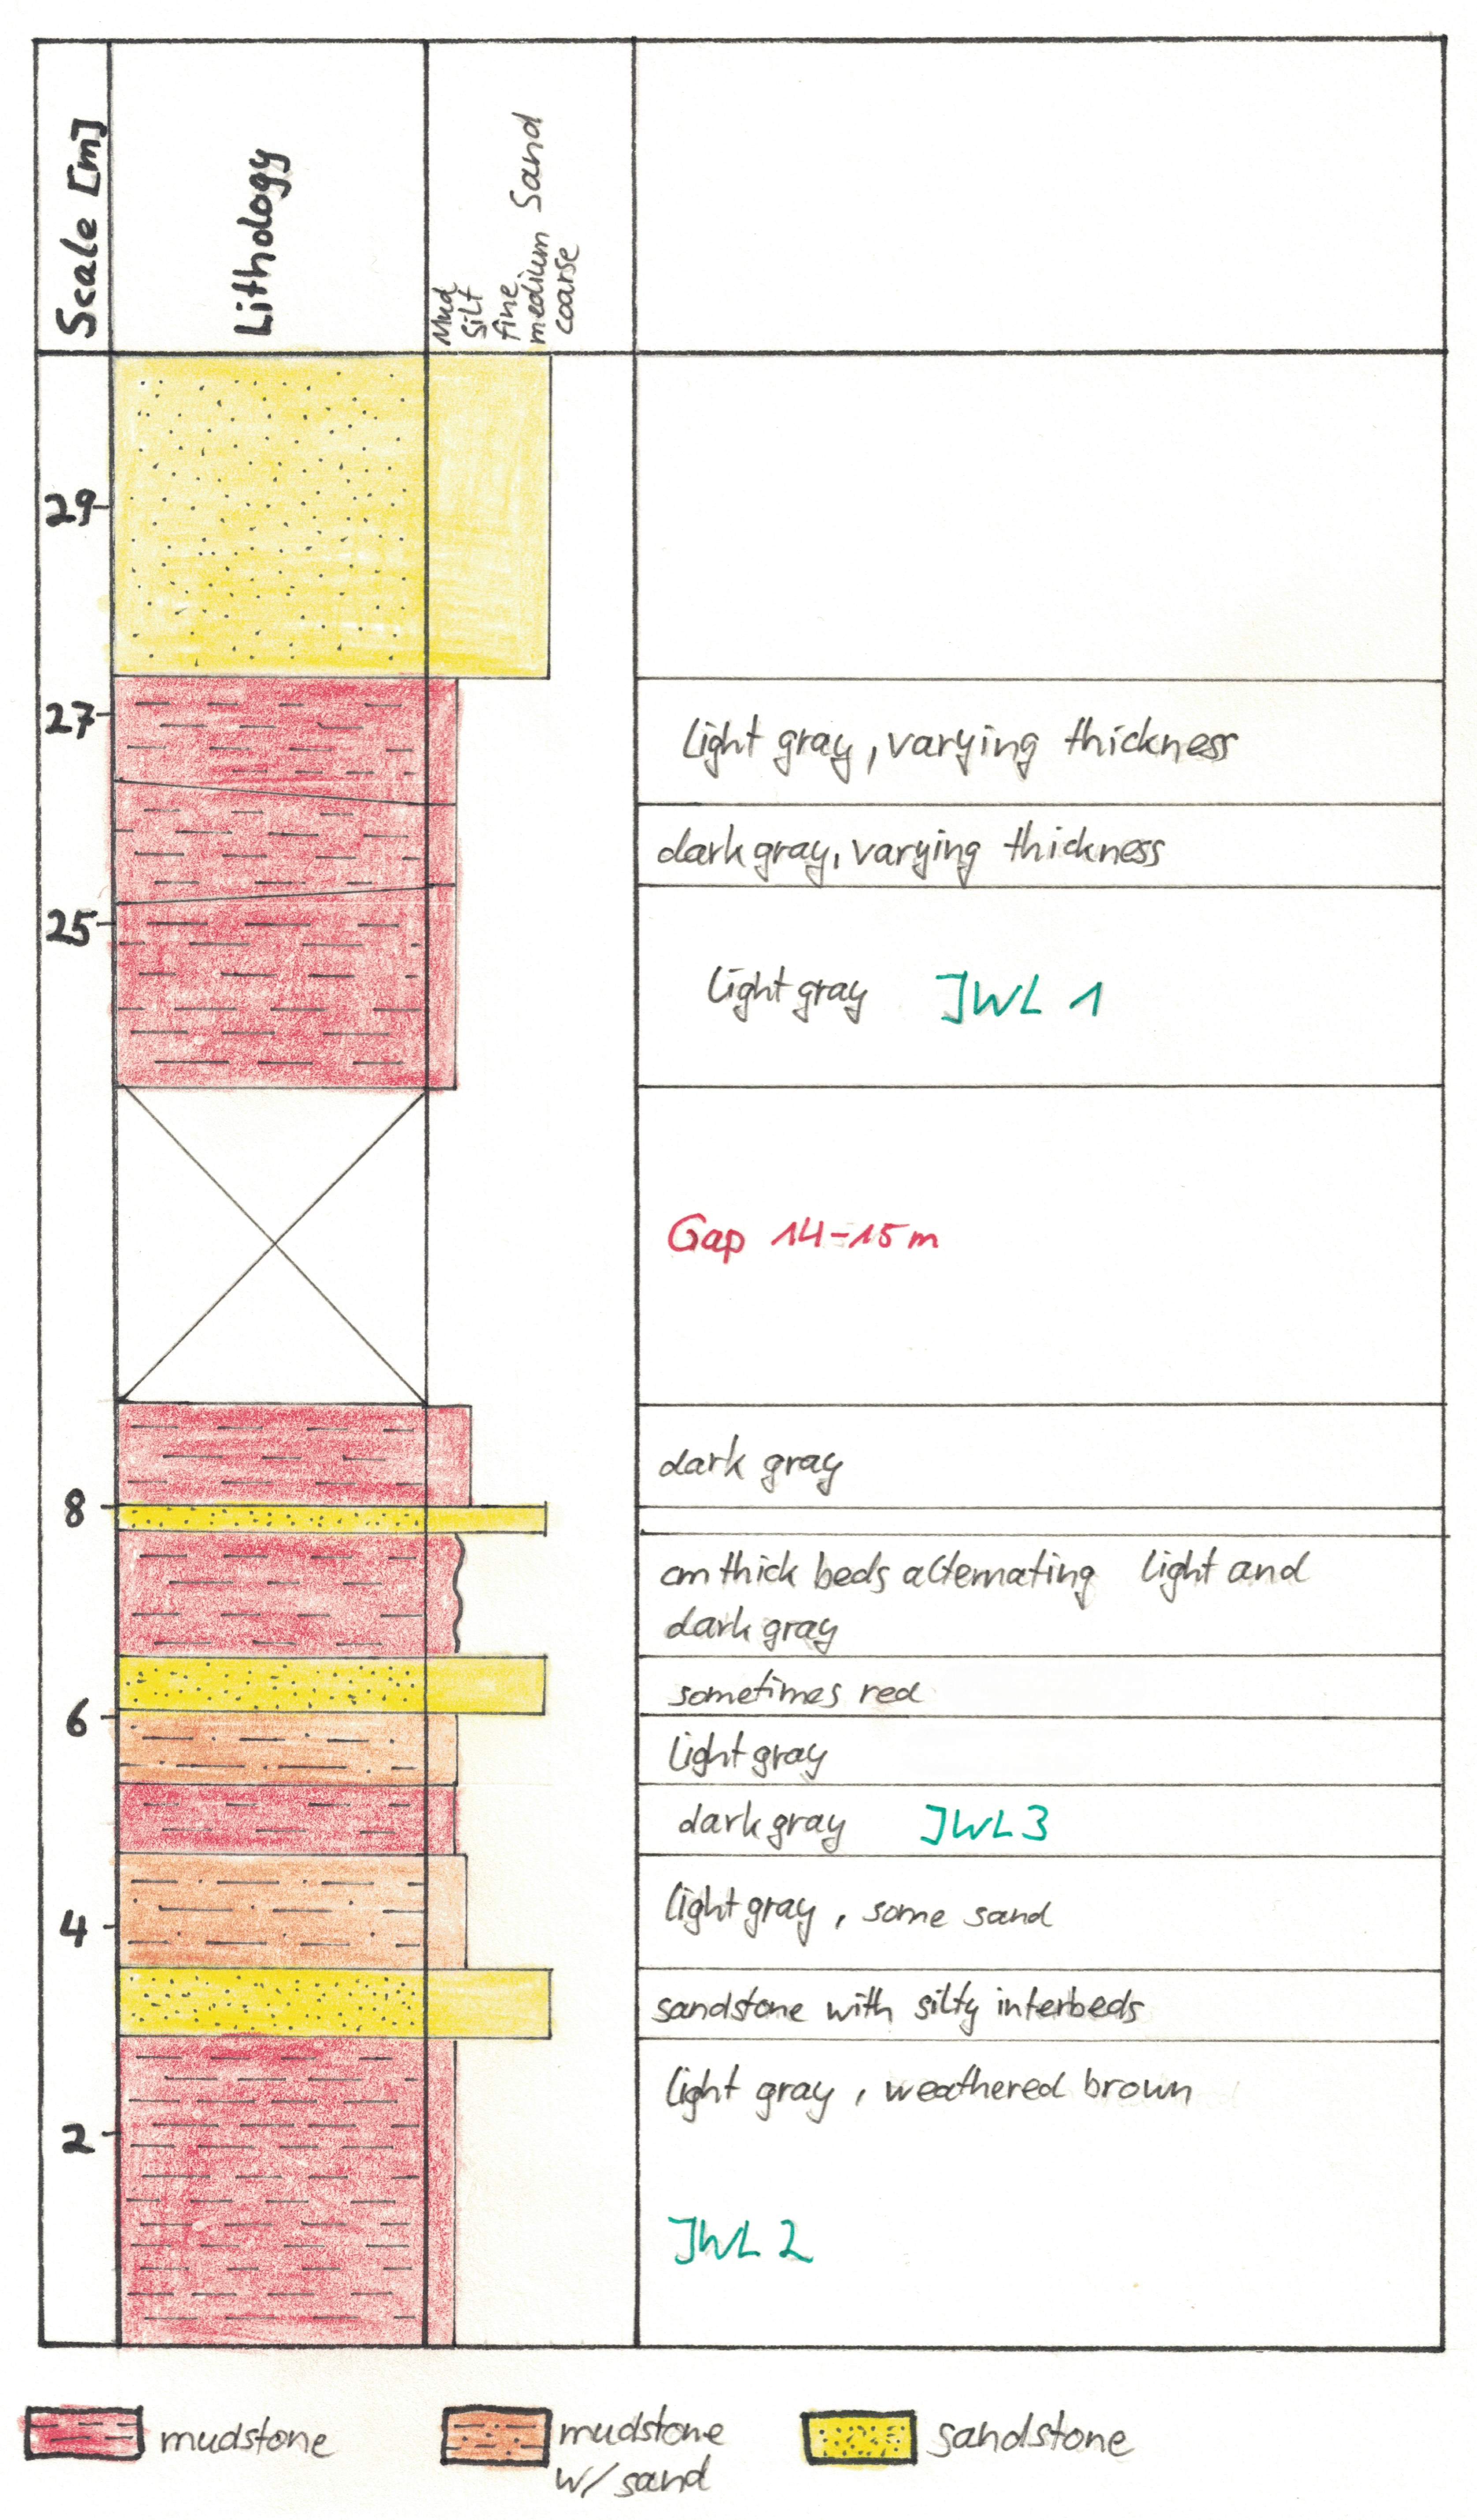
\includegraphics[width=0.5\textwidth]{img/L1_log.jpg}
    \caption{Stratigraphic log of the outcrop where samples JWL 1, 2 and 3 were taken. The outcrop
    is interrupted by an overgrown gap.}
    \label{fig:log_L1}
\end{figure}

% \begin{figure}
%     \centering
%     \fbox{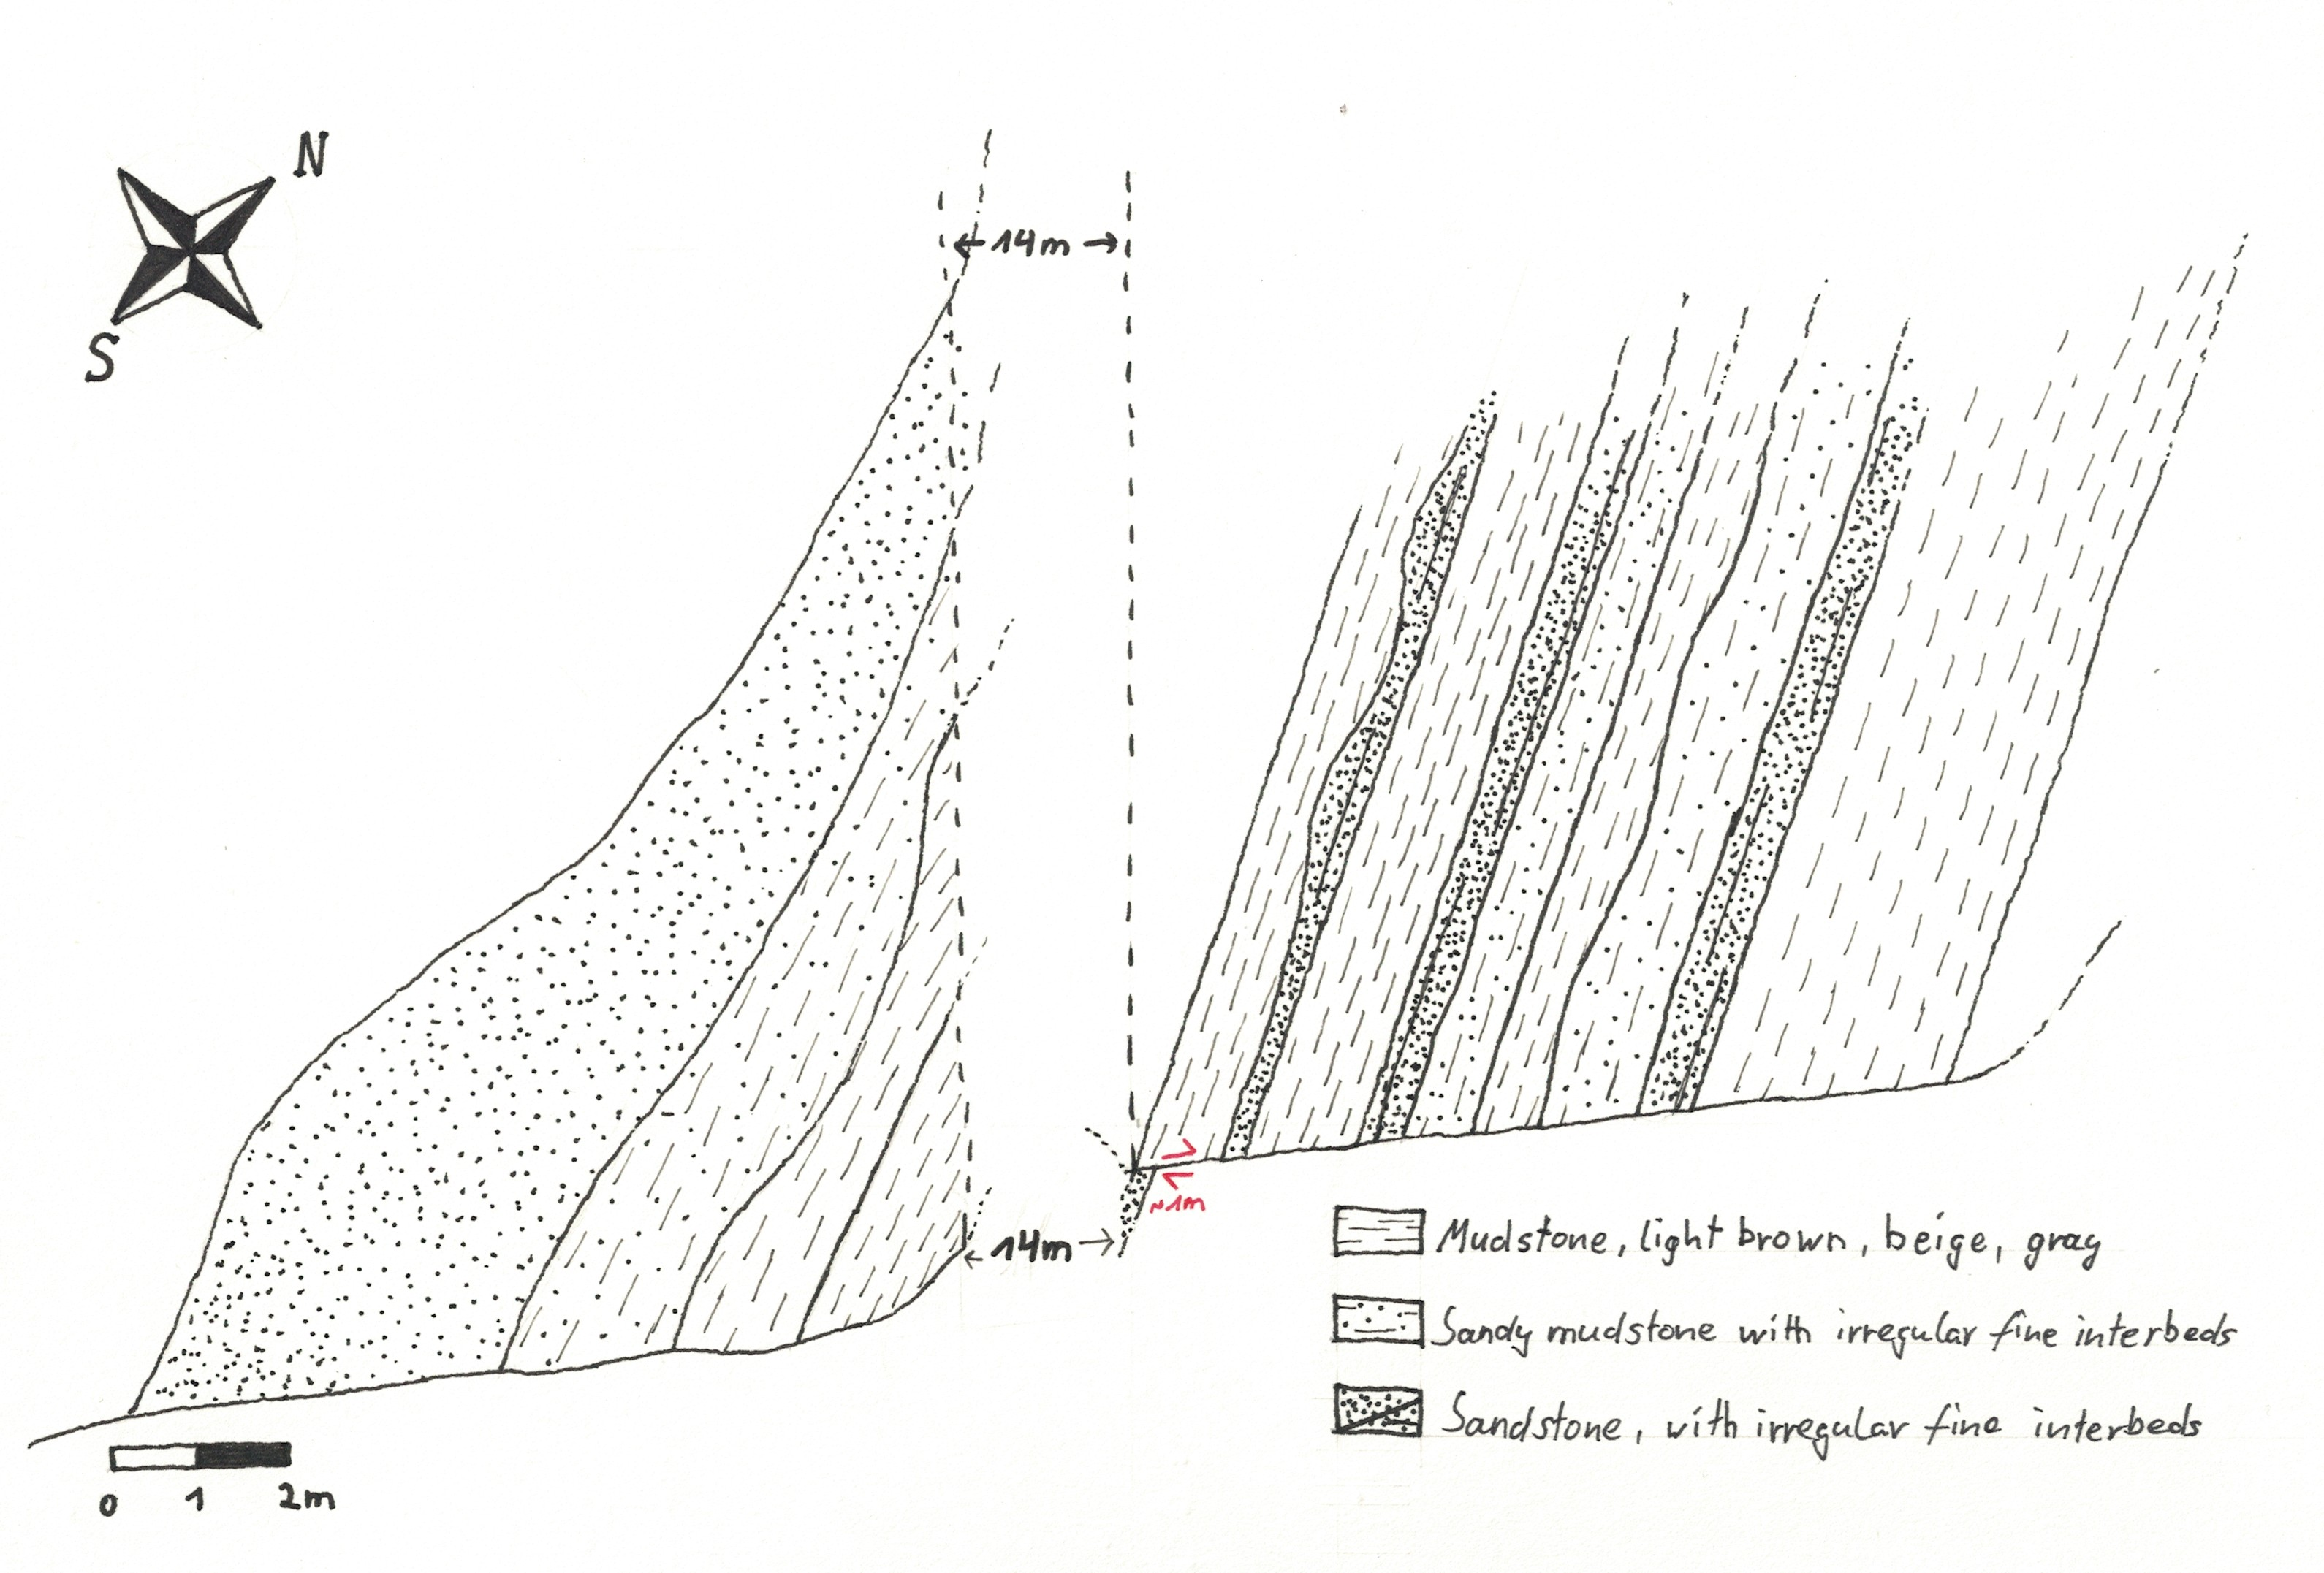
\includegraphics[width=0.95\textwidth]{img/loc_1_sketch.jpg}}
%     \caption{Sketch of the outcrop logged in \protect\cref{fig:log_L1}.
%     Bedding dips 200/65 in the right section. Dip is less clear in the more deformed left section.
%     Younging from right to left.}
%     \label{fig:loc_1_sketch}
% \end{figure}

\chapter{Conclusion}

\section{Summary}

\subsection{Methods}

We evaluated how directly applicable published (trace) element ratios are for the determination of the
depositional environment of sediments~\parencite{wei-2020,Worden_1996}. We used XRF, \ICPMS and IRMS to
obtain concentrations of the elements of interest. The uncalibrated XRF method proved too 
unreliable to obtain usable results.
The determination of Cl/Br proved difficult with \ICPMS. The published method for measuring halogens
\parencite{he_determination_2019} could not be reproduced successfully and even led to significant corrosion of the instrument. 
In contrast, the measurement of elements like Sr, Ba, and S worked reliably with the established
HF digestion method, and IRMS produced reliable results for \TOC.

We found that the thresholds for Sr/Ba published by \textcite{wei-2020} do not match the classification based
on the geological map (\textcite{Linth_Map}, \cref{fig:study_area}), while the S/TOC measurements work
with the published thresholds, especially those by \textcite{berner-raiswell-1983}.
Calibrating the thresholds to local conditions improves the results for Sr/Ba.
This calibration
requires certified standards of both depositional environments. For our study such certified
samples were not available, consequently we relied on the classification based on the geological map, 
excluding the obvious outlier JWL~1.
Because we relied on the existing classification to judge if the measured ratios give a reliable classification,
we cannot in turn use the obtained classifications to check if the existing classification is correct.

Overall, the S/TOC ratio provides a strong signal with our data. Sr/Ba separates the samples far less clearly,
and only with calibration. Therefore, it should be considered only when standards for calibration are
available, and as an auxiliary signal.

\subsection{Geology}

We were interested in whether some of the units mapped as \USM in our study area (\cref{fig:study_area})
contain marine layers or may be of marine origin altogether. 
Our data does not allow us to answer that question conclusively, but it strongly indicates that the sample JWL~1
originates from a marine layer.

JWL~1 was collected from a layer with clear evidence of tectonic deformation, and the entire subalpine molasse has been 
deformed and uplifted in the study area. This opens the possibility of the layer having been moved to its current
location by tectonics, rather than having been deposited in-situ. Our study focussed only on the
geochemical analysis of the samples, and cannot make statements about the geology of the study area.


\section{Outlook}

\subsection{Methods}

Throughout the study, the methods we used raised several questions for further inquiry.

\XRF did not yield reliable quantitative results, because the instrument was not calibrated and no standards to
calibrate individual measurements were available.
The instrument should be calibrated before any further measurements are conducted. 
Certified, powdered standards for the elements we are interested in (B, Br, Cl, Ga, S, Sr, Ba) are not readily available.
Therefore, a custom standard would have to be made.

The Cl and Br concentrations measure with \ambif\ digestion confirm that halogens are retained in the digestion cake
and transferred into solution with ammonia~\cref{fig:halogen-sensitivity}, otherwise the
measured counts should be close to 0.
Therefore, determining how to use this method without damaging the instrument and how to control for the excess Cl 
will allow the study of the Cl/Br ratio with \ICPMS as well.

With this expansion of the trace element ratios we could study, several natural next steps present themselves.
Repeating the \XRF measurements to obtain Cl, Br, B, Ga, Sr, Ba, S would establish whether the
calibrated method yields results comparable to \ICPMS. 
The additional data for B/Ga would allow studying that additional ratio, also extensively discussed by \textcite{wei-2020}.
Repeating the \ICPMS measurements for Cl/Br would provide cross-validation for the XRF data.

That one previously published ratio requires local calibration, suggests that 
these ratios may not generalize as well as suggested by \textcite{wei-2020}. \Cref{fig:sr-ba-wei} shows that there
is significant variability in the dataset used by \textcite{wei-2020}. 
Whether this variability is caused by samples coming from different areas, or whether there can be such large
variability within well constrained areas is an important question regarding the generalizability of these results.

\subsection{Geology}

Between geology and geochemistry rests the challenge of independently classifying samples as
marine or freshwater sediments, e.g. with microfossils \parencite{kempf_lower_2005}.
This independent classification would enable assessing 
the precision and recall of the element ratios as classifiers, as well as creating a standard to calibrate the
ratio thresholds to local conditions.

With a validated calibration dataset and the corresponding thresholds, a study of an
extended area of the subalpine molasse would be feasible. Studying a larger area could provide
insights how frequent misclassified beds occur in the \USM and \UMM.
In any large study, a few of the samples taken should still be classified independently to ensure
the local calibration remains adequate.

The results of our study provide additional information about the stratigraphy
of the outcrops we sampled. Open questions remain regarding the origin of the marine layer JWL~1.
Fieldwork should establish the nature of the currently overgrown, underlying layer, and 
whether there are signs
of fault movement indicating it layer may have been moved into place, or if it indeed
indicates a possibly short transgression to marine conditions.
The latter would also suggest that the sediment was deposited in shallow conditions, which
could explain the presence of glauconite in some areas \parencite{Linth_Text,nichols-sedi-2023}.

Several additional steps should be taken here:
\begin{enumerate}
    \item Sample the beds on both sides of the gap for additional classifications.
    \item Find bedrock in the gap to complete the log, and sample some of the beds.
    \item Identify and describe fault movement, if indicators exist.
    \item Study other outcrops that belong to this stratigraphic sequence for more data.
\end{enumerate}

\appendix

\chapter{Tables}

\begin{table}[h!]
\centering
\caption{Sr and Ba concentrations with errors and ratios from XRF measurements. 
The Compton ratio indicates 
reproducibility of the results. Values between 0.9 and 1.1 are good, 0.8 to 0.9 require
additional input to interpret quantitatively, and ratios below 0.8 can only be interpreted 
qualitatively.}\label{tab:sr-ba-table}
\input{temp/sr-ba-table.txt}
\end{table}

\begin{table}
\centering
\caption{Sr and Ba concentrations with errors and ratios from \ICPMS measurements. The BCR-2 standard should show
$337\pm 7$\,ppm Sr and $684\pm 5$\,ppm Ba.}\label{tab:sr-ba-icpms-table}
\input{temp/sr-ba-icpms-table.txt}
\end{table}

\begin{table}
\centering
\caption{S and TOC concentrations from XRF and IRMS with errors and ratios.}\label{tab:s-toc-table}
\input{temp/s-toc-table.txt}
\end{table}

\begin{table}
\centering
\caption{S and TOC concentrations from \ICPMS and IRMS with errors and ratios.}\label{tab:s-toc-icpms-table}
\input{temp/s-hr-icpms-table.txt}
\end{table}

\chapter{Declaration of AI use}

% Source: https://library.ethz.ch/en/scientific-writing/plagiat-und-kuenstliche-intelligenz-ki.html#declaration-of-use

\setlength{\parindent}{0pt}

\textbf{Microsoft Co-Pilot} was used for advanced auto-complete for the repetitive data visualizations in 
Jupyter, all suggestions were reviewed and corrected when needed (\cref{sec:results}).

\textbf{OpenAI ChatGPT} was used to revise the entire text for clarity and brevity. All suggestions were reviewed,
content-related suggestions were discarded, approximately 80\% of style suggestions were discarded.

\backmatter

\addcontentsline{toc}{chapter}{\bibname}
\printbibliography

\cleardoublepage

\begin{acknowledgements}
\addcontentsline{toc}{chapter}{Acknowledgements}
This thesis would not have been possible without the help of many people.
I would like to thank my advisor Vincenzo Picotti for giving this research
direction and his instruction in the field. 
My co-advisor Gregory De Souza for his guidance around all things chemical and frequent input
on research methodology and the scientific standards one should aspire to.
Corey Archer, Negar Haghipour and Natalie Seibel for their patient instruction and assistance in sample preparation
and measurement execution in the various lab methods we used.

Thank you!
\end{acknowledgements}

\end{document}